\documentclass[11pt]{article}

% --- Page layout ---
\usepackage[a4paper,margin=1in]{geometry}

% --- Fonts & micro-typography (standard journal look) ---
\usepackage[T1]{fontenc}
\usepackage[utf8]{inputenc}
\usepackage{lmodern}
\usepackage{microtype}

% --- Math, graphics, tables ---
\usepackage{graphicx}
\usepackage{amsmath,amssymb,mathtools}
\usepackage{gensymb}
\usepackage{tabularx}
\usepackage{float}

% --- Figures / captions ---
\usepackage[labelfont=bf,font=small]{caption}

% --- Algorithms (optional; keep if used) ---
\usepackage{algorithm}
\usepackage{algorithmic}

% --- Bibliography (author-year) ---
\usepackage[round,authoryear]{natbib}

% --- URLs and hyperlinks ---
\usepackage{xurl} % better line-breaking for URLs
\usepackage[dvipsnames]{xcolor}
\usepackage{hyperref}
\hypersetup{
  colorlinks=true,
  linkcolor=blue,
  citecolor=blue,
  urlcolor=blue,
  bookmarksdepth=4
}

% --- Misc (keep only if used in the paper) ---
\usepackage[none]{hyphenat}
\usepackage[]{placeins}
\usepackage{pifont}
\newcommand{\cmark}{\ding{51}}
\newcommand{\xmark}{\ding{55}}

\usepackage{tikz}
\newcommand*\circled[1]{\tikz[baseline=(char.base)]{
            \node[shape=circle,draw,inner sep=0.8pt] (char) {#1};}}

\usepackage[framemethod=tikz]{mdframed}
\usepackage{afterpage}
\usepackage{comment}
\usepackage{dirtytalk}

% --- Custom commands ---
\newcommand*\diff{\mathop{}\!\mathrm{d}}
\newcommand*\Diff[1]{\mathop{}\!\mathrm{d^#1}}

% --- Keywords environment (article class has none by default) ---
\newenvironment{keywords}{\par\small\noindent\textbf{Keywords:}\ }{\par\normalsize}

\title{\Large\bfseries Local and global synchronisation of persistent sub-national price cycles and the destabilisation of U.S. housing}

\author{
  Bazil Sansom\thanks{Warwick Business School, Coventry, CV4 7AL, UK. Email: \texttt{Bazil.Sansom@warwick.ac.uk}.}
}

\date{} % leave blank for submission; or set \date{\today}

\begin{document}
\maketitle
%%%%%\thispagestyle{empty}
%%%\setcounter{page}{1}
%%%%%%%%%%%%%%%%%%%%%%%%%%%%%%%%%%%%%%%%%%%%%%%%%%%%%%%%%%%%%%%%%%%%%%%%%%%%%%%%%

\begin{abstract}
%In this paper I introduce a number of novel wavelet based tools, applied to the nearly 50 years of available monthly state level price series (1975-2022), to empirically investigate the spatio-temporal dynamics of U.S. house prices across time and frequencies. I find: (i) Wavelet power spectrum analysis shows local markets across the U.S. exhibit striking but previously undocumented evidence of a permanent cycle component (with a preferred period of c.10 years) over the entire sample period. (ii) Novel instantaneous phase and amplitude based statistics show that a dramatic synchronisation of these permanent cycles after 1995, contributed to the subsequent \textit{national} house price boom-bust of the 2000s. (iii) using the spatial projection of instantaneous relative phase series as a new amplitude free approach to studying possible \say{ripple effects} at different time-scales, reveals a striking east-west travelling-wave pattern associated with the permanent cycle component in the data. This pattern closely resembling patterns typically observed in systems of locally coupled cycles. Taken together these results suggest a possible significant re-interpretation of the character of U.S. housing market instability in terms of the synchronisation of non-trivial local endogenous boom-bust dynamics.
In this paper I investigate the spatio-temporal dynamics of U.S. house price fluctuations at different time-scales over time using novel wavelet-based tools applied to nearly 50 years of available monthly state level price series (1975-2022). This yields interesting new insights. I find (i) wavelet power spectra show local markets across the U.S. exhibit striking and previously undocumented evidence of a permanent cycle component over the entire sample period (with similar preferred periods of c.10 years); (ii) instantaneous phase coherence shows that a synchronisation of these existing permanent cycles after 1995, contributed to the subsequent \textit{national} house price boom-bust of the 2000s; (iii) the spatial projection of instantaneous relative phase series (a novel amplitude free approach to studying possible \say{ripple-effects} at different time-scales) reveals for the first time a striking repeating East-West travelling wave pattern associated with the permanent cycle component identified in the data. This pattern closely resembling patterns characteristically observed in systems of locally coupled cycles. Taken together these results suggest a possible re-interpretation of U.S. housing market instability in terms of the synchronisation of non-trivial local endogenous boom-bust dynamics with spatial spillovers between markets - if local markets are in endogenous boom-bust regimes, both a \say{ripple-effect} and national boom-bust could arise endogenously out of spatial spillovers, and common shocks could drive persistent and increasing co-movement between markets.
\end{abstract}

\begin{keywords}
\textit{housing cycles; synchronisation; ripple effect/spatial diffusion; housing bubbles}
\end{keywords}

%%%%%%%%%%%%%%%%%%%%%%%%%%%%%%%%%%%%%%%%%%%%%%%%%%%%%%%%%%%%%%%%%%%%%%%%%%%%%%%%
\section{Introduction and Motivation}

The central role the national U.S. housing market boom-bust of the $2000$s seemed to play in the Global Financial Crisis and subsequent recession, has generated huge and ongoing research and policy interest in the dynamics of house prices and the sources and propagation of housing market instability. 

A view widely shared among academics and policymakers is that the 2000s boom period saw U.S. house prices depart from their fundamental values, leading to distortions and ending in the price correction that eventually precipitated the crisis \citep{Bernanke2010}. 

While the \textit{national} boom-bust of the $2000$s is unprecedented since the Great Depression era, at the \textit{sub-national} level the U.S. has a long history of housing market instability \citep{Glaeser2013}. Evidence of sub-national house price cycles goes back at least to Homer Hoyt’s classic study of Chicago land prices \citep{Hoyt1933} in which Hoyt documented real estate cycles between 1830-1933 with a 17-20 year periodicity. Moreover regional boom-bust episodes were not uncommon in the decades immediately preceding the national boom of the 2000s and had been widely documented in the literature \citep{Case1992,Case1993,Case1988,Riddel1999,Wheelock2006,Shiller1990}.

%\begin{figure}[tbp]
%\centering
%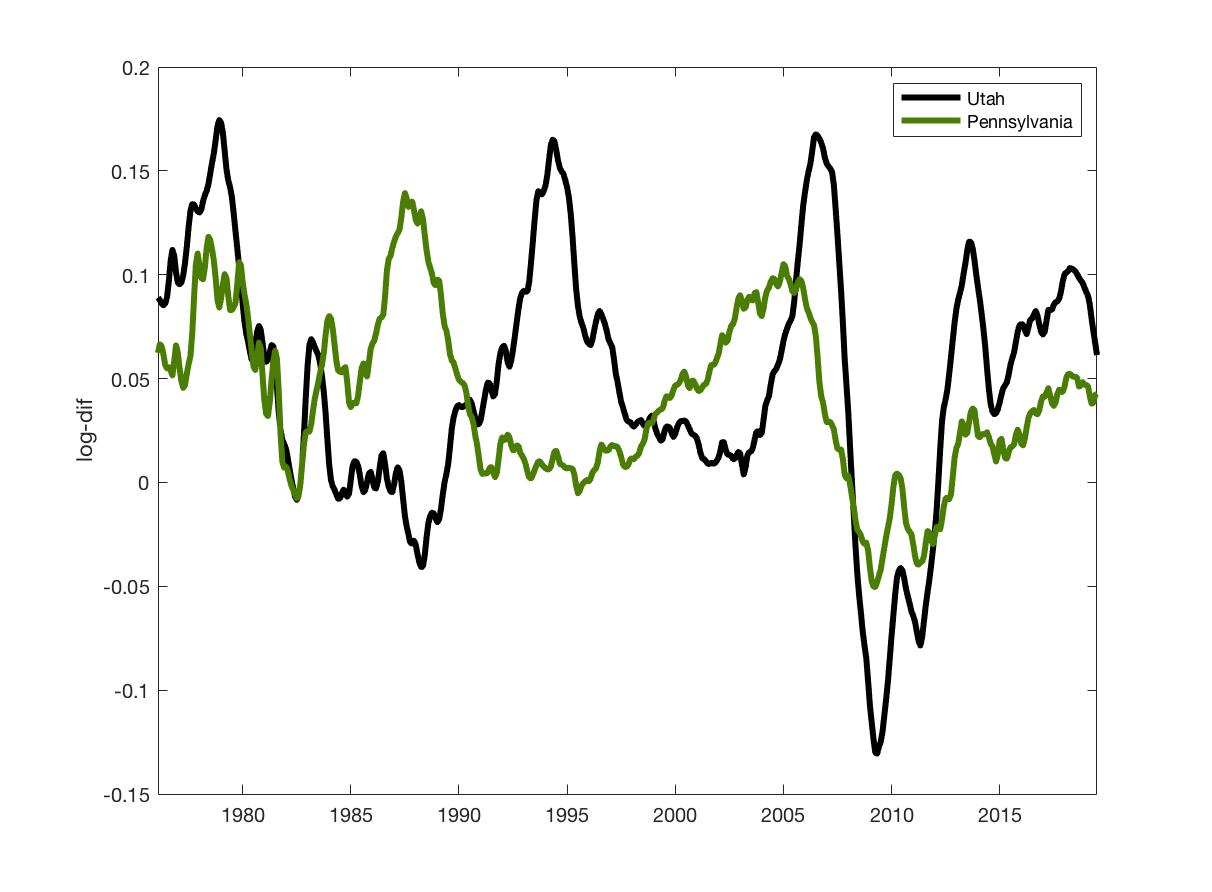
\includegraphics[width=0.97\linewidth]{figs/Fig_example_price_series.jpg}
%\caption{This figure presents examples of state level house price series illustrating the repeated boom bust cycles experienced by many markets prior to the national housing boom-bust of the 2000s}
%\label{cycles}
%\end{figure}

These experiences have motivated a key debate over whether house prices are %locally 
stable but subject to shocks; or can exhibit temporary bubble episodes, uncoupling from fundamentals over extended periods \citep{Shiller1990, Mikhed2009, Clark2011, Abraham1996}.  

Given that historically boom-bust largely averaged out at the national level, a natural conclusion was that this volatility - whether driven by shocks or bubbles - was in any case, local and idiosyncratic \citep{DelNegro2007}.

%A natural assumption is that house prices reflect some combination of both market specific (e.g. city or state specific) and of common national factors (such as monetary policy).

This had important implications for housing finance (leading to a perceived risk diversification opportunity from pooling mortgages from different parts of the country \citep{BISCommitteeontheGlobalFinancialSystem2005,Coval2009,Cotter2015}); and for monetary policy (since the effects of a policy shock depend on the initial distribution of regional housing market conditions; moreover heterogeneous regional shocks are outside of the scope of monetary policy making \citep{DelNegro2007,Fratantoni2003}). % Fuss 2012? Brady 2014?

Meanwhile the national boom-bust of the 2000s is widely believed - by the same logic - to have reflected the emergence of significant common \textit{national} drivers in house price formation during this period (a wide range of factors have been put forward including interest rates \citep{Campbell2009,Glaeser2013a,Himmelberg2005}; mortgage credit and subprime lending \citep{DellAriccia2012,Favilukis2016,Levitin2012,Mian2009,Pavlov2009,Wheaton2008}; speculation and irrationality \citep{Barlevy2011,Bayer2011,Bayer2016,Case2005,Case2003,Lee2011,Shiller2005,Wheaton2008, Burnside2016}; and international capital flows \citep{Favilukis2013,Favilukis2016}).%  generating systematic risk.

%It has been previously documented in the literature (see e.g. \cite{DelNegro2007} for an early study), that prior to the “national bubble” period of the 2000s, house price variation was dominated by idiosyncratic movements (consistent with local shocks or local bubbles), but that a common component dominated house price movements from the mid-2000s (consistent with the significant influence of a national shock or bubble during this period).

%Similarly, systematic studies by a recent empirical literature that employs time-localised tests for explosive dynamics (argued to be the hallmark of an unstable bubble, rather than equilibrium adjustment process \cite{Phillips2015}) find evidence of a history of widespread local bubbles in most markets prior to the national boom-bust (consistent with the “lots of local bubbles” conjecture of Greenspan [ref]), but finds bubbles arose simultaneously across the US during the 2000s, and burst even more synchronously in 2006-7 (in line with the national bubble hypothesis) \cite{Hu2018}.

It is interesting to notice however, not only had many regional markets experienced similarly dramatic boom-bust episode prior to the 2000s, but also that the succession of boom-bust in some markets seem to more resemble an ongoing cycle than isolated events. %(Fig.\ref{cycles} shows two example price series illustrating the sort of repeated cycles experienced in many markets). 
This apparent continuity in house price dynamics that can be observed at a sub-national level raises the question whether local cycles are best understood as an irregular episodic process (mainly a response to persistent exogenous shocks, or else temporary bubble dynamics), or could they instead reflect an endogenous mechanism which produces recurrent boom-bust phenomena? %This in turn raising interesting questions regarding the role of "local" vs. "national" factors in the national boom-bust of the 2000s.

%This apparent continuity in house price dynamics when observed at a sub-national level, seems to raise interesting questions both regarding the dynamic character of housing boom-bust; and regarding the relationship between local cycles, and national price fluctuations:

%\vspace{3mm}

%\begin{itemize}
%\item 
 %[should include refs for these different possibilities?]
%\vspace{3mm}
%\item 

%Were markets sufficiently independent, recurrent endogenous boom-bust might still be expected to average out at the national level.\footnote{I.e. if the phase of cycles in different markets were uniformly distributed, then despite cyclicality of individual markets, national housing aggregates would be stable.} 

%However housing markets across the U.S. are of course subject to a range of significant common national factors (e.g. interest rates, credit conditions and inflation may be important examples). What is more, spatial dependence and spillovers are important themes in real estate economics and a number of empirical studies document evidence of some form of spatial dependence among U.S. markets \citep{Baltagi2014,Dolde1997,Pollakowski1997,DeFusco2013,Brady2011,Kuethe2011,Vansteenkiste2007,Holly2010}. Other non-spatial direct links between markets may also play a role (relevant studies for the U.S. include \cite{Pollakowski1997,Hernandez-Murillo2017,Malone2017,Zhu2013}). 

%In the context of persistent cycle dynamics, these sorts of common shocks, or local dependencies between markets could easily give rise to co-movements contributing to persistent national price fluctuations.\footnote{Housing markets across the U.S. are of course subject to a range of significant common national factors (e.g. interest rates, credit conditions and inflation may be important examples). What is more, spatial dependence and spillovers are important themes in real estate economics and a number of empirical studies document evidence of some form of spatial dependence among U.S. markets \citep{Baltagi2014,Dolde1997,Pollakowski1997,DeFusco2013,Brady2011,Kuethe2011,Vansteenkiste2007,Holly2010}. Other non-spatial direct links between markets may also play a role (relevant studies for the U.S. include \cite{Pollakowski1997,Hernandez-Murillo2017,Malone2017,Zhu2013}). } % need refs for noise driven sync? local coupling driven synch?

Moreover, if housing market fluctuations during the 2000s when observed at a sub-national market level can be understood as the continuation of recurrent local boom-bust dynamics, this would also raise the question: to what extent the national boom-bust during this period could be understood as a shift in relationship among existing non-trivial cycle dynamics in regional markets vs. (as is generally assumed) directly reflecting some persistent common shock or national drivers of a temporary bubble at this time? %[What about question of whether the crisis could have synchronised persistent cycles?]

%In this paper I empirically explore these questions. I deploy complex \textit{time-frequency} methods applied to monthly state level house price data since January 1975 in order to: 
%\vspace{2mm}
%\begin{itemize}
%\item
%Assess the evidence for the existence and historical timing of persistent cycle episodes in house price fluctuations at the state level across different markets.
%\item
%Study the phase-synchronisation among state level cycles to see how this has varied or evolved over time.
%\item
%Study spatial patterns in the phase (timing) of state level  cycles in order to assess any important spatial segmentation or propagation patterns between markets.
%\end{itemize}
%\vspace{2mm}

%Regarding the character of local housing cycles: 
Of course these alternative dynamic regimes may not necessarily always be readily distinguished in empirical data:
a series of random shocks could generate a ‘cycle’ in the sense of successive periods of expansion and contraction (analogous to modern business cycle theory) \citep{Bracke2013}; alternatively if markets are \say{bubbly} enough (i.e. if bubbles easily emerge but eventually burst) this explosiveness could be the engine behind a cycle formed by a sequence of bursting bubbles \citep{Evans1991,Shi2007,Shi2017}. %The multiple bubbles hypothesis is empirically supported by evidence of temporarily explosive dynamics \cite{Shi2017,Hu2018,Greenaway-mcgrevy2015,Pavlidis2018} - the time series signature of an unstable bubble process (see \cite{Phillips2015} for an overview).

Whether driven by successive shocks or bubbles, if explained by this sort of episodic process, housing cycles might recur, but would in either case, be fundamentally \textit{irregular} and \textit{unpredictable}. By contrast, as recently argued for example by \cite{Beaudry2020} in the business cycle literature, although irregular cycles may \textit{also} arise out of the interplay between exogenous shocks and endogenous cycle dynamics, we might nevertheless expect time series generated by this sort of shock buffeted system with non-trivial deterministic dynamics, to exhibit evidence of a preferred period.  %(wherein the system is buffeted by exogenous shocks, but where the deterministic part of the system admits a limit cycle). %- a dynamic possibility that has been shown to arise in a number of recent housing market models \cite{}. 

%As a result these alternative possible dynamic regimes may not necessarily always be readily distinguished in empirical data.

One approach to distinguishing between different sorts of cycle dynamics, is thus to inspect the time-series spectral density. This of course depicts the importance of cycles of different frequencies in explaining the data over some given sample period (which should be sufficiently long) and can reveal the underlying periodic tendency of even a noisy cycle process \citep{Beaudry2020}.\footnote{It is well known that if the spectral density of a time series displays a significant peak at a given frequency, this is an indication of recurrent cyclical phenomena at that frequency - consistent with endogenous cycle dynamics but something not shared by a locally stable equilibrium reverting process where fluctuations are generated only by exogenous shocks; or by unstable periodically collapsing bubble processes \citep{Evans1991}.} 

Whilst powerful for revealing the time-series signature of different sorts of qualitative dynamics, a key drawback of a pure frequency domain approach however, is that it averages over the entire sample period.

This is a serious limitation since: cycle episodes may be transient (if their amplitude quickly decays); or the onset of cyclicality may occur at a particular time (in response to a structural change); or cycle characteristics (duration, magnitude) may change over time. Where cycles interact, cycle frequencies and/or phase may converge over time or synchronise under common shocks \cite{Pikovsky2001}. % what about importance of instantaneous phase? 

%What is more, the phase relationships between cycles in different markets may vary over time: spatial propagation of fluctuations should give rise to a systematic spatial pattern, but this pattern of lead-lags between markets may depend on specific historical shocks to particular markets. Alternatively, as already mentioned, in the context of persistent cycle dynamics synchronisation could easily increase as a result of common shocks, or direct interactions between markets. In this setting spatial patterns may form, and clusters of synchronised markets may also arise and merge.

%This range of possibilities motivates the development of tools more a more dynamic framework with which to explore the history of U.S. house price dynamics over the available sample period.

In this paper I introduce and deploy new methods suitable for studying these sorts of possible dynamics, based on the \textit{complex continuous wavelet transform} \citep{Aguiar-Conraria2014}.
%which has become widely employed in the analysis of noisy and non-stationary dynamical systems.  % which has been shown to be useful in identifying cyclical signals in data from noisy dynamical systems
%Continuous wavelet transform more robust to noise: \cite{Mallat1998,Torrence1998,Cazelles2008}
Wavelet analysis performs the estimation of the spectral characteristics of a time series as a function of time, revealing how the different periodic components of the time series change over time \citep{Aguiar-Conraria2014} with the ability to identify trends or abrupt shifts in cyclic dynamics (leading it to become widely employed in the analysis of noisy and non-stationary dynamical systems).  %The wavelet transform allows an optimal \textit{time-frequency} decomposition of the variance of a time series %- it is as though estimating the spectral density as a function of time - and has the ability to identify not only time variation, but also abrupt shifts in cyclic dynamics \cite{}. 
Complex wavelet transforms also provide a convenient \textit{phase-amplitude} decomposition - separating timing from magnitude.%, facilitating in a multivariate setting, the quantification of phase and amplitude contribution to correlation between time series.

%With these 
I exploit this combined \textit{time-frequency} and \textit{phase-amplitude} decomposition 
%provided by the complex continuous wavelet transform, 
as the basis for new methods with which to study U.S. housing cycle dynamics across \textit{frequencies}, over \textit{time} and \textit{space}, using state level monthly house price data since January 1975 (c.50 years of data).

%applied to spatially granular (state level) monthly house price data since January 1975 (c.50 years of data) in order to study U.S. housing cycle dynamics across \textit{frequencies}, over \textit{time} and \textit{space}.
%Applying wavelet based methods to monthly state level house price data since January 1975, I am able to 

These relatively advanced empirical tools allow me to first evaluate whether any U.S. housing markets have exhibited evidence of fluctuations with a preferred \textit{period}; then to study the time evolving \textit{phase} relationship (an amplitude free measure of relative timing) between cycle components with similar periodicity in different markets, quantifying the historical evolution both (i) of the overall synchronisation among cycles across the U.S., as well as (ii) the spatial pattern in the relative timing (phase lead/lags) of state level cycles across the country.

%This systematic spatio-temporal pattern, and the continuity between the historical period of "local" and "national" housing market instability, at once challenge both the view that housing market instability was idiosyncratic prior to the national boom-bust (since the timing of ); and the subsequent emphasis on the search for an aggregate explanation in the search for a smoking gun following the national boom-bust of the 2000s.%, able to explain the simultaneous run up and collapse of prices in markets across the country. 


This study contributes to the literature in a number of ways: where the empirical bubble literature employs tests for time-localised zero frequency explosive behaviour in U.S. house price series \citep{Kivedal2013,Phillips2011a,Zhou2005,Bolt2014}, I look for evidence of a preferred period - consistent with an endogenous mechanism which produces recurrent
boom-bust phenomena.\footnote{Another possibility of course is that some markets are not switching but permanently in an unstable Evans bubble type regime \citep{Evans1991}. However if bubble period duration has some regularity, this would imply - unlike Evans bubbles - that bubbles not only build, but also end endogenously.} 

While housing market co-movement \cite{DelNegro2007}, and possible \say{ripple effects} have long been studied and theorised \citep{Meen1996,Meen1999}, this is to the best of my knowledge the first study to consider the possibility for housing market \say{ripple effects} to arise out of endogenous boom-bust dynamics, as well as the first study to use an instantaneous phase based approach making it possible to obtain a consistent time-evolving multivariate measure of synchronisation and to study time evolving \say{ripple effects} at different frequencies (i.e. temporal-scales).\footnote{Note this approach is suitable not only for empirically analysing the relationship between cycles with a preferred period, but can also provide a powerful new tool for studying the endogenous propagation of specific local shocks at different time-scales.} %While I study permanent cycle components in the data, this approach could also provide a powerful tool for studying the endogenous propagation of specific local shocks at different time-scales.


\cite{Flor2017} also use wavelets to study regional U.S. house prices cycles, however this work starts from performing spatial aggregation based on a clustering method employing a measure of similarity that does not separate phase and amplitude, and that is neither frequency specific nor time specific. I introduce more flexible informative methods that by contrast provide time varying frequency specific measures separating phase and amplitude information, suitable for analysing patterns in spatially disaggregated data (thus for studying space in a smoother/more continuous way).

%Methods I introduce here also extend wavelets methods available for economic and financial time series analysis in ways likely to be useful for business cycle analysis and for analysis of spatial time series. by introducing multivariate instantaneous phase based approaches to studying co-movement and 

Key findings include: (i) evidence of persistent cycle components with a similar preferred period of c.10 years in markets across the U.S. over the entire historical sample period (ii) the contribution
from these cycle components in state level markets to mean house price variation at the national
level was significantly moderated prior to the 2000s by the
phase-shifts between markets, but a dramatic increase
in synchronisation after 1995 contributed to the subsequent
national boom-bust; (iii) however while synchronisation increases, the phase-shifts between these cycles in different markets describe a clear non-random spatial pattern (persisting over the entire sample period and multiple cycles) resembling a repeating \textit{traveling-wave} across the country - with cycles synchronised north-south, but travelling east-west, closely resembling patterns typically observed in systems of locally coupled cycles. %rather than a system primarily dominated by the spatial propagation of exogenous shocks.

This study thus makes an important contribution to our understanding of U.S. housing market fluctuations. Both evidence of a preferred period in state level price fluctuations, and the smooth systematic spatial pattern revealed in the timing of this cyclic components across markets, shows a significant systematic component to the underlying dynamics. This, combined with the apparent continuity between the historical period of \say{local} and \say{national} housing market instability at once challenges both the view that housing market instability was idiosyncratic prior to the national boom-bust (since cyclic components may have averaged out, but are revealed to have been far from random in temporal or spatial dimensions); as well as the subsequent emphasis on common factors in the search for a smoking gun following the national boom-bust of the 2000s (since it suggests the simultaneous run up and subsequent collapse in prices in markets across the U.S. partly reflected the \textit{synchronisation} of \textit{existing} non-trivial \textit{local} endogenous boom-bust dynamics - rather than e.g. a reduction in the variance of local shocks and increase in the variance of national shocks \citep{DelNegro2007}). Taken together these results suggest a significant re-interpretation of U.S. housing market instability.

%as spatially coupled local endogenous boom-bust subject to local and common shocks.

%More recent work by \cite{Flor2017} applies the wavelet based clustering tools provided by \cite{Aguiar-Conraria2011} to study U.S. house prices at the sub-national level between 2001-2013. This involves first aggregating markets into clusters based on measure of combined phase and amplitude similarity (no separation of cycle similarity and cycle synchronisation) across frequencies (not time-scale specific), then considering bi-variate phase differences between clusters. While employing similar methodological foundations, choice of methods and sample period mean the significant phenomena I document here, are missed by their study.


%I assess the existence and historical timing of cyclical episodes; compare the characteristics of cycles in different markets over time%- I focus in particular on the \textit{period} of cycles in different states
%; quantify the overall synchronisation among cycles across the U.S. at each time-step; and finally look at the time-evolving spatial pattern in the relative timing of state level cycles.%  over the last c.50 years.

%What is more the continuity in this spatio-temporal patterns between the historical "local" and "national" instability periods 

%o prior to the "national bubble" era (rather than the idiosyncratic character local fluctuations have been assumed to have). Taken together these results suggest a possible significant re-interpretation of U.S. housing market instability.

%Taken together these results are consistent with significant intrinsic dynamics and the importance of spatial links between markets, and suggest a possible significant reinterpretation of U.S. housing market instability.
%in terms of the synchronisation of national boom-bust.

%are consistent significant intrinsic cycle dynamics and an important role for . Spatial patterns confirm the importance of spatial dependence in housing market dynamics and show for the first time a striking "ripple effect" in U.S. markets. However combined with evidence of ongoing boom-bust with a relatively stable cycle period, this spatial pattern suggests a possible spatially coupled cycle hypothesis distinct from the spatial diffusion of local shocks widely studied in the real estate literature.

%This allows me to assess the existence and historical timing of cyclical episodes, and to compare \textit{period} and \textit{phase} similarity of cycles across different markets. Combined with spatial information, it also allows me to assess whether there have been any spatial patterns in the relative timings of cycles across different markets. 

%- Standard business cycle methods require specifying the relevant range of periodicities to focus on.

%I use wavelet power spectrum analysis – which has been shown to be useful in identifying cyclical signals in data from noisy dynamical systems - as a simple method by which to study whether regional house price dynamics exhibit any evidence of persistent or permanent cyclicality, to assess the existence and historical timing of cyclical episodes

%The wavelet transform allows an optimal \textit{time-frequency} decomposition of the variance of a time series - it is as though estimating the power spectrum as a function of time. Wavelets analysis has the ability to identify not only time variation, but also abrupt shifts in cyclic dynamics.

%In a noisy endogenous cycle setting, wavelets analysis should have some power to distinguish the signature of the cycle dynamics in the signal from the spectrum of the stochastic environment in which it is embedded (which will depend on the specific process but will not have a preferred period) allowing me to assess the existence and historical timing of cyclical episodes, and to compare the \textit{period} of cycles in different markets.

%I then introduce instantaneous phase based methods (also obtained via wavelet transform) in order to study both the overall synchronisation of cycles across the U.S., and the temporal relationship between cycles in different markets. The use of instantaneous phase series allows me to study whether cycles have become more synchronised over time, and assess whether there are any significant spatial patterns in the timing of cycles.

%I then introduce a new statistic for quantifying the phase synchronisation in a multivariate setting.

%Wavelets analysis has the ability to identify not only time variation, but also abrupt shifts in cyclic dynamics. 

%The dynamic view provided by this time-frequency approach is important since cycle episodes may be temporary, cycle frequencies may not be stable over time (for example in the business cycle literature it has been argued cycle periods may be getting longer \cite{}, or in coupled cycle systems cycle frequencies may converge over time \cite{Pikovsky2001}), which markets are leading or lagging may change depending on specific shocks to different markets, local clusters of synchronised markets may form, or merge over time.

%- and for complex wavelets additionally allows a \textit{phase-amplitude} decomposition. This allows me to assess the existence and historical timing of cyclical episodes, and to compare \textit{period} and \textit{phase} similarity of cycles across different markets. Combined with spatial information, it also allows me to assess whether there have been any spatial patterns in the relative timings of cycles across different markets. 


%The multiple bubbles hypothesis is empirically supported by evidence of temporarily explosive dynamics \cite{Shi2017,Hu2018,Greenaway-mcgrevy2015,Pavlidis2018} - the time series signature of an unstable bubble process (see \cite{Phillips2015} for an overview).

%I employ wavelet analysis, which is widely used in the analysis of noisy dynamical systems.

%In this paper I use complex \textit{time-frequency} methods in order to study the time varying character, similarity, synchronisation and spatial patterns in the timing of housing cycles across the U.S. since 1975. 

%In this paper, I use wavelet power spectrum analysis – which has been shown to be useful in identifying cyclical signals in data from noisy dynamical systems - as a simple method by which to study whether regional house price dynamics exhibit any evidence of persistent or permanent cyclicality. This is based on the projection of house price series into the time-frequency plane where its spectral content can be followed over time.

%In this sort of setting however, wavelets analysis should have some power to distinguish the signature of the cycle dynamics in the signal from the spectrum of the stochastic environment in which it is embedded (which will depend on the specific process but will not have a preferred period).

%The wavelet transform allows a \textit{time-frequency} decomposition of the variance of a time series - it is as though estimating the power spectrum as a function of time.


% this would raise questions over the current assumption that the national run up in house prices was principally driven by an exogenous aggregate shock or temporary national bubble.
%\end{itemize}
%\vspace{3mm}

%Besides common national factors that effect all markets, another source of co-movement in housing markets may be direct links between markets. Spatial dependence and spillovers are well established themes in real estate economics. 

%If housing markets exhibit recurrent cycles, is there any particular spatial pattern in the timing of these cycles?

%The increased co-movement of house prices is widely documented. Is this driven by common factors; local spillovers. Associated with . One possible source is common factors; another is spatial dependence. What has contributed to the increased co-movement of house prices?

%The multiple bubbles hypothesis is empirically supported by evidence of temporarily explosive dynamics \cite{Shi2017,Hu2018,Greenaway-mcgrevy2015,Pavlidis2018} - the time series signature of an unstable bubble process (see \cite{Phillips2015} for an overview).

%As recently argued by Beaudry et al. \cite{Beaudry2020} irregular fluctuations may also emerge as the interplay between exogenous shocks and endogenous cycles - a phenomena that has been shown to arise in a number of theoretical settings/house price models. % In this sort of setting wavelets analysis should have some power to distinguish the signature of the cycle dynamics in the signal from the spectrum of the stochastic environment in which it is embedded (which will depend on the specific process but will not have a preferred period). 

%While on the one hand housing market boom-bust is argued to have been idiosyncratic, at the same time spatial dependence and spillovers are well established themes in the real estate literature.

%In this paper I investigate: state level house price cycles; the (phase) synchronisation of these cycles over time; spatial distribution of/patterns in the timing/phase of these cycle phases in order to identify the spatial propagation or segmentation of housing cycles across U.S. states.


% - If the cycles were independent, they might still average out. However common shocks, or links between markets could give rise to persistent co-movement.
% - On the one hand local housing market volatility assumed to be idiosyncratic, on the other hand spatial dependence and spillovers are a well-established theme in the real estate literature.

% Not well treated by dynamic factor model approach, which does not allow for phase-differences between the common cycles in different markets; and generally assumes local cycles are independent - local diffusion or contagion are thus ruled out as a source of strong cross-sectional dependence/nationwide co-movement.
% Spatial econometric models meanwhile require weak cross-sectional dependence. CCM method first strips out what covariance can be captured by a common factor, then studies residual spatial dependence. In some cases dynamic spatial effects are considered through the introduction of time-lagged spatial lag, but in either case spatial patterns are not revealed, rather averaged across links and over a sample period or window.

%Study housing cycles as a continuous process; co-movement among regional cycles over time; and spatial patterns in their co-movement.

%Standard methods do not make a good treatment of time (does not allow phase-differences between cycles); spatial correlation does not reveal spatial patterns.

%A common and natural hypothesis is that housing market fluctuations may have both a national and local components \cite{DelNegro2007}.  Many studies attempt to estimate these using a latent factor decomposition approach - a panel of price growth rates is decomposed into loadings on a low-dimensional vector of latent factors, and a vector of market-specific variation satisfying weak cross-sectional dependence.  Even studies interested in spatial effects, first control for strong cross sectional dependence, and study spatial patterns in the residual weakly cross-sectionally dependent variation \cite{Baltagi2014, Holly2010}. 

%However while common shocks may be one source of co-movement, significant co-movement could also arise from the propagation of market-specific shocks, contagious bubbles, or from the interaction of local intrinsic dynamics. Thus while such a variance decomposition is always possible, care must be taken in its interpretation as common shocks rather than the result of endogenous co-movement generated by the interactions between different markets (a concern raised for example in production network context by \cite{Carvalho2019b}).

%While the propagation of of local disturbances may be a source of strong cross-sectional dependence, it may also give rise to temporal patterns in the timings of these fluctuations.


%The wavelet transform allows a \textit{time-frequency} decomposition of the variance of a time series - it is as though estimating the power spectrum as a function of time - and for complex wavelets additionally allows a \textit{phase-amplitude} decomposition. This allows me to assess the existence and historical timing of cyclical episodes, and to compare \textit{period} and \textit{phase} similarity of cycles across different markets. Combined with spatial information, it also allows me to assess whether there have been any spatial patterns in the relative timings of cycles across different markets. 

%Wavelets analysis has the ability to identify not only time variation, but also abrupt shifts in the cyclic dynamics. The dynamic character of this approach is important since cycle episodes may be temporary, cycle frequencies may not be stable over time, spatial synchronisation patterns may change depending on local shocks to different markets. % Need to say they also allow local propagation as source of comovement..?

%The question of how the co-movement of US markets has changed over time has been previously addressed in the literature, based on a variety of different methods, datasets, and sample periods. Methodologically these studies rely variously on: simple correlation analysis \cite{Landier2017,Kallberg2014}  quantifying the tendency of prices across different markets to co-move from one time-step to the next; cointegration and error correction methods \cite{Yunus2013}  to test whether price differences between markets are mean reverting - thus whether regional housing cycles move around/share a common stochastic trend in the ‘long-run’; latent factor models \cite{DelNegro2007}  or simple multivariate regression frameworks  \cite{Cotter2011} as a way to try and estimate the relative importance of common (respectively latent or observed) national (vs. idiosyncratic local) factors in house price movements; and spatial econometric models \cite{Abate2016}  in order to assess the co-movement of contiguous markets. In all cases these methods are made dynamic through the use of rolling-windows or recursive estimation. 

%All these studies seem to report a trend to increasing co-movement across subnational markets starting well before the housing and sub-prime crisis of 2006-8.  However 

% \vspace{3mm}

%\begin{itemize}
% \item The time-domain methods on which these studies rely are uninformative with regard to the character of common price dynamics driving these results - co-movement may vary across frequencies as well as over time thus it is important, in general, to question whether the trend to increased comovement is driven by long-run trend, cycles, or short-run volatility components of the data.
 %\vspace{3mm}
 %\item Correlation based methods are sensitive to both phase and amplitude variation, moreover rolling window based methods employed to make correlations dynamic are subject to a number of problems or biases in the presence of cyclical dynamics, and/or time varying volatility or phase-differences (as will often be the case).
%\end{itemize}
% \vspace{3mm}

%By contrast the phase-amplitude decomposition and time-frequency localisation made possible by the \textit{complex wavelet transform} provides the basis for a scale-specific analysis of time-varying co-movement that distinguishes phase and amplitude contributions and is robust to non-stationarity. 

%This also both provides the basis for a much more continuous measure, and is more robust to noise, than methods for quantifying phase-synchronisation based on the joint distribution of binary state variables (such as expansion/contraction \cite{Harding2006, Harding2003}; or sign based deviations from trend \cite{Bordon2013,Gogas2009,Mink2012}  widely employed in the existing business cycle literature.

%These allow me to identify common cycle components across state level markets and disentangle and quantify the contribution to aggregate house price variance from the time-varying amplitude envelope and time varying phase-synchronisation of these cycles as observed at the state level. %Wavelets analysis has the ability to identify not only time variation, but also abrupt shifts in the cyclic dynamics.

The rest of this article is organized as follows: in Section \ref{Literature} I review relevant empirical literature; Section \ref{Methodology} introduces some key methodological building blocks for the analysis presented; Section \ref{Data} briefly explains my data; Section \ref{Analysis} presents my analysis and results. In Section \ref{Discussion} I discuss the meaning and significance of my results; Section \ref{conclusion} concludes.


%%%%%%%%%%%%%%%%%%%%%%%%%%%%%%%%%%%%%%%%%%%%%%%%%%%%%%%%%%%%%%%%%%%%%%%%%%%%%%%%

\section{Related literature} \label{Literature}

% May not be possible to separate out this neatly into three subsections, but I should cover all of these. Cycle vs. bubble question. Increased co-movement question. Spatial dependence and propagation question.

\subsubsection{Housing cycle dynamics}


The character and causes of house price fluctuations have been and remain hotly debated. An important question %regarding the character of house price dynamics 
(at the local and the national level), has been whether prices are stable but subject to random independent shocks, or may exhibit unstable bubble dynamics \citep{Abraham1994,Clark2011,Mikhed2009,Shiller1990}.
%Few now would argue that house price movements are orderly and driven entirely by obvious changes in fundamentals.  Nevertheless 

While economic theory suggests a variety of market imperfections and/or ‘alternative’  behavioural assumptions that may amplify fundamental shocks,\footnote{Key examples are credit-constraints \citep{Ortalo-magne2006,Stein1995},  search market externalities \citep{Diaz2013,Wheaton1990}, (policy) constraints on the elasticity of supply \citep{Glaeser2007}, and e.g. backward-looking expectations schemes \citep{Capozza2002,Case1988}.} enormous house price increases and subsequent crashes have led many researchers to test for the presence of speculative bubbles.

The empirical bubble literature reports evidence of temporarily explosive dynamics (argued to be the time series signature of an unstable bubble process rather than equilibrium adjustment in response to a shock  (see \cite{Phillips2015} for an overview)).\footnote{Where property prices are determined not only by economic fundamentals, but driven either by the rational expectation of a future gain from future price increases \citep{Flood1990},  or by irrationally optimistic expectations \citep{Shiller2000,Vissing-jorgensen2004}, house prices will follow an explosive process. A substantial empirical literature exploits this feature of non-fundamental asset price components as the basis for formal bubble tests - framed both within the well known present-value model \citep{Diba1988,Hall1999,Homm2012,Pavlidis2016,Phillips2011a,Phillips2011} and e.g. trend-following behaviour \citep{Bolt2014} hypothesised in the behavioural asset market literature.} % Time-localised zero frequency unit root \cite{}} 

Econometric studies of U.S. markets find national house price series followed an explosive process during the 2000s boom period %consistent with e.g. a temporary rational bubble or period of “irrational exuberance” 
\citep{Kivedal2013,Phillips2011a,Zhou2005,Bolt2014}. %While many studies focus on aggregate US house price developments, 
Meanwhile similar studies of regional house price series both (i) identify a long history of such explosive episodes at the local market level (consistent with multiple \say{local} bubbles prior to the 2000s); and (ii) confirm that explosive episodes were geographically widespread during the 2000s (consistent with a \say{national bubble} during this period) \citep{Shi2017,Hu2018,Pavlidis2018}.

While the bubble identification literature presents compelling evidence of significant time-localised explosive dynamics in regional house price series (i.e. at the zero frequency), the succession of such explosive episodes exhibited by many markets raises the question whether these markets are really switching occasionally between stable and temporarily explosive dynamics as hypothesised, or are rather in an endogenous cycle regime due to a locally unstable, or only weakly stable equilibrium. 

Thus while the empirical bubble literature employs tests for time-localised zero frequency explosive behaviour \citep{Kivedal2013,Phillips2011a,Zhou2005,Bolt2014}, I test for evidence of a preferred period - consistent with an endogenous mechanism which produces recurrent
boom-bust phenomena.\footnote{Another possibility of course is that some markets are not switching but permanently in an unstable Evans bubble type regime \citep{Evans1991}. However if bubble period duration has some regularity, this would imply - unlike Evans bubbles - that bubbles not only build, but also end endogenously.}

The possibility of these sorts of endogenous dynamics have been shown to arise in a number of different \textit{theoretical} house price model settings \citep{He2015,Bolt2014,Burnside2016, Kouwenberg2015, Eichholtz2015, Dieci2012, Dieci2016,Lingling2009,Baptista2016,Geanakoplos2012,Sommervoll2010,Defusco2017, Chia2017, Diks2016}. However \textit{empirical} studies of whether house prices actually exhibit evidence of these sorts of periodic dynamics seem to be lacking (for the U.S. and for housing in other economies).% 

%[Some studies must have looked at Fourier transform? Spectral density?]

%Many bubble studies study individual episodes?

%[Good methods may not have been readily available? What I do here compared to all this]

\subsubsection{Housing cycle co-movement and spatial diffusion}

A common and natural hypothesis is that housing market fluctuations may reflect both national and local factors. Spatial dependence and spillovers, or other local links between markets may also be a source of co-movement across markets and are well established themes in real estate economics. 

Some studies attempt to estimate unobserved common factors using a latent factor decomposition approach \citep{DelNegro2007} - a panel of price growth rates is decomposed into loadings on a low-dimensional vector of latent factors, and a vector of market-specific variation (satisfying weak cross-sectional dependence).\footnote{This approach is also widely employed in the study of international house price cycles \cite{}} %[Weak law of large numbers: \cite{Forni1998} ... idiosyncratic components average out]. 

This latent factor model approach typically does not allow for phase-shifts between common components (that may e.g. naturally arise as a result of local propagation% or differing response times
), and by assuming local components are independent from each other, precludes the meaningful study of bilateral linkages between markets as a source of co-movement across all markets.

%However while common shocks may be one source of co-movement, significant co-movement could also arise from the propagation of market-specific shocks, contagious bubbles, or from the interaction of local intrinsic dynamics. Thus 

While such a variance decomposition is always possible, care must be taken in its interpretation and the assumption that co-movement represents common shocks rather than endogenous co-movement generated by the interactions between different markets (a concern raised for example in the analogous context of production networks by \cite{Carvalho2019b}).

Investigating the role of local links in co-movement presents some methodological challenges however. 

Local dependencies between markets - especially spatial dependence - are well established themes in real estate economics. However standard spatial econometric models may fail in the presence of strong cross-sectional dependence (generally requiring weak forms of cross-sectional dependence, in the sense that dependence decreases sufficiently quickly along the spatial dimension \citep{Pesaran2011}). 

What is more, the spatial coefficients yielded by these models provide only a measure of contemporaneous local correlation averaged across links (adjacent pairs based on the introduction of a spatial adjacency matrix) and across the sample period or window. Even where dynamic spatial effects are considered through the inclusion of a time-lagged spatial correlation \citep{Chudik2011,Baltagi2014}, the resulting spatial coefficients in either case provide only a measure of average spatial dependence, and do not provide any information on spatial patterns.

Some studies employ methods designed to accommodate both common factors and local links between markets as a sources of correlation \citep{Pesaran2006,Pesaran2011}: first using variation that can be captured by a common component to control for strong cross-sectional dependence, then studying residual spatial dependence %across the idiosyncratic components 
using a standard spatial econometric model (e.g. spatial autoregressive model) (applications in a U.S. housing market context include \cite{Holly2010,Baltagi2014}). 

Although studies employing this approach still find significant spatial dependence \citep{Holly2010,Baltagi2014}, this methodology also starts from the assumption that covariance that can be captured by common components is driven by common factors. What is more, the standard spatial model estimated based on residual covariance, again only provides a test of spatial dependence based on average correlations. %only evidence of spatial dependence (but find a significant spatial effect, even after controlling for State specific real incomes, and allowing for a number of unobserved common factors).

The considerable existing empirical \say{ripple effect} literature - which researches spatial propagation of house prices - has mostly relied on cointegration tests for convergence,  asking whether markets move around/share a common stochastic trend in the \say{long-run} (i.e. whether they move together over time exhibiting mean-reverting “spreads”) and rely on restrictive assumptions on the order of integration of time series. 

The existence of a \say{ripple effect} (in the simple sense of spatial propagation of disturbances) might occur however even in the absence of long-run convergence; what is more even where convergence occurs cointegration tests do not measure the synchronisation or reveal the spatio-temporal pattern of short run adjustments or provide a dynamic view of the data.%, but a test of long-run comovement over the sample period. 

Indeed studies for the U.S. in fact report mixed but limited evidence of convergence for U.S. markets and this has been argued to cast doubt on the existence of a \say{ripple effect} for the U.S. \citep{Clark2009,Pollakowski1997,Holmes2011,Zohrabyan2008,Holly2010,Gupta2012,Gil-Alana2014}.\footnote{By far the largest literature on the \say{ripple-effect} is for the U.K. \citep{Meen1996,Meen1999}, but ripple-effects have been tested for in many countries.}

While these methods all provide time-averaged estimates of co-movement, some studies have employed rolling-windows or recursive estimations in order to address the question of how the co-movement of U.S. markets has changed over time.\footnote{simple correlation analysis \citep{Kallberg2014,Landier2017}% quantifying the tendency of prices across different markets to co-move from one time-step to the next
; cointegration and error correction methods \citep{Yunus2013}%  to test whether price differences between markets are mean reverting - thus whether regional housing cycles move around/share a common stochastic trend in the ‘long-run’
; latent factor models \citep{DelNegro2007} or simple multivariate regression frameworks \citep{Cotter2011} as a way to try and estimate the relative importance of common (respectively latent or observed) national (vs. idiosyncratic local) factors in house price movements; and spatial econometric models \citep{Abate2016}  in order to assess the co-movement of contiguous markets.} However, not only are there a number of potential issues with employing rolling-windows with many of these approaches, but also none of these time domain approaches to studying time-varying co-movement provide the spectral information or phase-amplitude decomposition possible with wavelet analysis.

By contrast with %a latent factor model approach, 
these traditional econometric approaches, I use a time-frequency and phase-amplitude decomposition to first empirically identify cycle components\footnote{No assumptions are required as for turning point based methods widely used in the business cycle literature, and to some extent housing cycle analysis.} in different markets; then study time evolving phase-relationships (lead-lag) between similar cycles (cycles with similar frequency) in these markets in terms of their overall phase-synchronisation and in terms of the specific spatial pattern of phase-differences between them.

%This allows me to separate the role of frequency components vs. phase relations

Strong cross-sectional dependence does not pose a problem (as it does for spatial econometric models) for this approach of studying the time evolving phase lead-lags between cycles with similar frequencies, which allows me to separate the amplitude and phase contributions to changing correlations. My phase-differences approach provides a very intuitive approach to studying \say{ripple effects}, what is more the scale-specific analysis provides for the first time a study of \say{ripple-effects} at specific time-scales.


%and study the phase-adjusted similarity between cycles in different markets; then study the phase synchronisation and pattern of phase-differences between markets at cycle frequencies identified as empirically relevant.

%the role of amplitude vs. phase in changing correlation among markets over time. SAY MORE/SOMETHING ELSE

%Given my focus on the pattern of phase-lead lags, strong cross-sectional dependence does not pose a problem (as it does for spatial econometric models) and the simple spatial projection of the instantaneous phase of the common cycle component that I introduce allows a rich elucidation of  the exact pattern of relationships.% (not just an average across all adjacent pairs).
%\footnote{Although I also consider the phase-coherence of adjacent markets.}

%What is more, the instantaneous phase based approach that I introduce allows me to study the development of overall synchrony and of spatial patterns with good temporal resolution.

%Window chosen optimally for scale of analysis... this not the case with moving-window estimations of time-domain models! Hence spurious variation in correlation using rolling windows.


%has been previously addressed in the literature, based on a variety of different methods, datasets, and sample periods. 

%Methodologically these studies rely variously on: simple correlation analysis \cite{Kallberg2014,Landier2017}% quantifying the tendency of prices across different markets to co-move from one time-step to the next
%; cointegration and error correction methods \cite{Yunus2013}  to test whether price differences between markets are mean reverting - thus whether regional housing cycles move around/share a common stochastic trend in the ‘long-run’; latent factor models \cite{DelNegro2007} or simple multivariate regression frameworks \cite{Cotter2011} as a way to try and estimate the relative importance of common (respectively latent or observed) national (vs. idiosyncratic local) factors in house price movements; and spatial econometric models \cite{Abate2016}  in order to assess the co-movement of contiguous markets. 

%In all cases these methods are made dynamic through the use of rolling-windows or recursive estimation. 


\subsubsection{Wavelets methods in economics and housing}

Wavelets analysis is widely employed in a range of applied sciences,\footnote{Wavelet analysis is extensively used in physics, neuroscience, epidemiology, ecology, climate science, seismology, signal processing, etc.} and has become increasingly employed in economics \citep{Crowley2007,Soares2011,Aguiar-Conraria2014,Gallegati2014}, especially in studying cyclical properties of economic and financial time series, and their cyclical comovements.

%Univariate analysis?

%Continuous wavelet transform more robust to noise: \cite{Mallat1998,Torrence1998,Cazelles2008}


A growing number of studies employ wavelet coherence (or related measures such as \textit{\say{cohesion}} \citep{Rua2010}) to provide a pairwise measure of correlation in the time-frequency domain \citep{Crowley2008,Aloui2014,Reboredo2017,Klarl2016,Li2015,EuropeanCentralBank-WorkingGrouponEconometricModelling2018,Flor2017,Aguiar-Conraria2011}. These have been generalised to the multivariate context simply by averaging over all possible pairs \citep{Rua2012,Kurowski2018}. These measures provide a combined measure of phase and amplitude correlation.

One problem with this approach may be that areas of low power may be similar between spectra of different series. %\footnote{In general it is not a good idea to average spectrum of different series...} 
What we really want to know about is common areas of high power. In a study of business cycle synchronisation Aguiar-Conraria and Soares \citep{Aguiar-Conraria2011} first apply a dimension reduction approach (SVD) to extracted components corresponding to the most important common patterns (areas of high power) between the wavelet spectra, then they compute a measure of distance between the two spectra.

Their measure of distance again takes into account both the real and the imaginary part of the wavelet spectrum, thus provides a combined measure of phase and amplitude correlation %(high similarity implies two series share the same high power regions and also that their phases are aligned). This measure of similarity 
and is based on a comparison of the whole time-frequency matrix. Similarity is thus maximised when two series consistently (over the entire sample period) share the same high power regions and their phases are aligned.% consistently over the entire sample period.

Pairwise instantaneous phase-difference provides a %frequency specific 
dynamic measure of phase lead-lag that has become increasingly used since introduced to economics by  \citep{Soares2011}. %This is a pure phase measure. 
%\footnote{While economic applications stress the size of the phase difference (smaller phase-difference -> more synchronous)  the stability of phase-difference over time (phase-locking) also provides a relevant measure of synchronisation.}  %and in phase vs. anti-phase 
However the methodological question of instantaneous phase synchronisation in a multivariate context, although studied by the wider synchronisation literature \citep{Pikovsky2001,Rosenblum2001,Rodrigues2015,Arenas2008,Schroder2017}, has not to the best of my knowledge been previously addressed in economics. % (although studied by the wider synchronisation literature \cite{Pikovsky2001,Rosenblum2001,Rodrigues2015,Arenas2008,Schroder2017}).

%To the best of my knowledge, while instantaneous phase-differences are employed in the economics literature, a multivariate measure of instantaneous phase-synchronisation (or phase coherence) has not previously been employed. One reason for this may be that caution should be exercised with respect to risk of looking at phase-coherence where this not associated with important aspects of variance of series being studied.

It provides significant advantages however, over the \textit{concordance index} methods \cite{Harding2002,Harding2003,Harding2006,Mink2012,Bordon2013} - based on the fraction of time that two series spend in the same binary (expansionary or contractionary) phase - widely employed to study phase-synchronisation in the business cycle literature (housing cycle applications include \citep{Jackson2008,Alvarez2009,Hirata2013a,Miles2015a}). Because only discrete distances between turning points are used to approximate underlying phase-differences, valuable temporal information is lost. What is more since the dating of turning points (based on commonly used algorithms such as \cite{Bry1971}) may also be imprecise in the presence of noise and complex spectral content, and require assumptions on cycle periods, these indexes also lack spectral precision.

Given increasing adoption of wavelet based methods for the study of co-movement, and wide interest in phase synchronisation in business cycle literature, it is surprising that the imaginary part of the wavelet transform has so far been largely overlooked.\footnote{For example a recent report from ECB Working Group on Econometric Modelling \citep{EuropeanCentralBank-WorkingGrouponEconometricModelling2018} uses wavelet power spectra in order to assess cyclical properties of growth series, and wavelet coherence to assess bi-variate comovements, but resorts - in the very same paper - to binary indicator based \textit{concordance} approach in order to measure bi-variate and multivariate phase synchronicity.}
The instantaneous measure of overall phase-synchronisation in a multivariate setting that I introduce in this paper seems likely to find wide relevance in a range of other applications.

%Some applications of wavelet based methods to the study of housing market cycles have also been made \cite{Flor2017}. 

In what is by far the closest study to my own, \cite{Flor2017} borrow the method introduced by \cite{Aguiar-Conraria2011} in order to study U.S. regional housing market sychronisation (they study MSA level data). 

They first perform the clustering routine (as per \cite{Aguiar-Conraria2011}: SVD based dimension reduction, then pairwise distances reflecting a combined measure of phase and amplitude similarity). They then look at (i) the power spectrum of the average price series for each cluster; %\footnote{Price growth rate averaged over the identified clusters.} 
and (ii) the wavelet coherence and instantaneous phase-differences between clusters and the national house price index series.\footnote{Some weighted mean of regional data.}

One simple but important difference between our studies is that they only study data between 2001-2013 (c.10 years of data compared to the c.50 years of data I study here).\footnote{It is not clear why they do not use full available historical time-series dimension given on the one hand the problem of edge effects, and on the other hand the good temporal resolution provided by the transform} 
A sample of this length of course makes it impossible for them to study lower frequency dynamics, and is only really suitable for analysis of variance in a 2-3 year periodicity band. As a result the c.10 year cycles I identify and study here is out side the scope of their analysis.

As above, their measure of synchronisation used in the primary step of cluster assignment, is a measure of combined phase and amplitude correlation; and %over the entire time-frequency matrix - i.e. they 
clusters markets that have both areas of similar power and phase over the entire sample period. They provide neither a measure of national synchronisation, nor detail on the spatio-temporal pattern in the timing of cycles.

In contrast to this,  I estimate instantaneous cycle frequency %(based on \textit{spectral ridge} identification) 
and compare cycle frequencies across different markets over time; I study separately (i) areas of common high power (phase-adjusted similarity of cycles) and (ii) the phase-synchronisation among markets at this common cycle frequency with an emphasis on how these (may) have changed over time. Finally I study detailed time evolving spatio-temporal patterns in the timing of house price cycles across the U.S.

%and phase similarity of cycles separately study the phase-adjusted 

%use the simpler approach of averaging power spectra in order to obtain information on common areas of high power across multiple markets (information about the phase, which depends on the imaginary part, is lost when we take the absolute value (Eq.\ref{eq:wps})); I introduce multivariate phase-coherence in order to assess changing synchronisation over time. Spatial projection to obtain detailed spatio-temporal information. They do not provide a measure of national synchronisation. The clustering approach they take means we don't have detailed spatial information.

%I am interested in (i) quantifying phase synchronisation for a specific frequency component and (ii) observing how this may have changed over time; (ii) 


%By comparison, I use local \textit{spectral ridge} identification as an estimate of instantaneous frequency and compare cycle frequencies across different markets; then having identified cycles of very similar frequency across markets, I look at the evolution of the instantaneous phase-coherence of these cycles over time.


%\cite{Kurowski2018} employ a concordance index approach (even whilst using bi-variate phase-differences). They also use a 

%---

%Wavelets analysis has become increasingly employed in economics. Examples include: .... power spectrum in order to assess cyclicality of macroeconomic time series \cite{};% coherence in order to assess spectral structure of co-movement over time \cite{}.

%business cycle synchronisation studied by \cite{Aguiar-Conraria2011} using approach that then borrowed by Flor and Klarl \cite{Flor2017} to study U.S. regional housing market sychronisation.

%It links to and improves substantially on the \textit{concordance index} approach \cite{Harding2003,Mink2012,Bordon2013} that has become widely employed in the business cycle literature (based on the fraction of time that two series spend in the same binary (expansionary or contractionary) phase identified using turning-points). Because only discrete distances between turning points are used to approximate underlying phase-differences, these indices lack time-resolution, dating of turning points may be poor in presence of noise and complex spectral content, lacks spectral precision.


%By far the closest study to my own is that of Flor and Klarl \cite{Flor2017} who also use a wavelets based approach to study housing cycle synchronisation across U.S. markets (they study MSA level data). They borrow from Aguiar-Conraria \cite{Aguiar-Conraria2011} a metric for measuring the distance between a pair of given wavelet spectra (using the singular value decomposition of power spectrum matrix to extract time-frequency regions of common high power) allowing the construction of a dissimilarity matrix and cluster analysis.

%The look at the phase-difference between clusters and national house price index (but make no meaningful analysis of phase-coherence among cycle).

%One important difference between our studies is simply that they only study data between 2001-2013 (c.10 years of data compared to the x.50 years of data I use in this study).\footnote{A curious choice given the on the one hand the problem of edge effects, and on the other hand the good temporal resolution provided by the transform} 
%A sample of this length of course makes it impossible for them to study lower frequency dynamics, and is only suitable for analysis of variance in a 2-3 year periodicity band - hence they do not identify the c.10 year cycles I find in my own study.

%Meanwhile, the measure of synchronisation they borrow from Aguiar-Conraria \cite{Aguiar-Conraria2011} is based on a pairwise measuring of distance between wavelet spectra for different series (using the singular value decomposition of power spectrum matrix to extract time-frequency regions of common high power). This is used to construct a dissimilarity matrix and perform cluster analysis in order to identify groups of markets whose power spectra share key features. 


%\subsubsection{Anything missing}

%Turning point based methods ().

%GVAR approach \cite{Vansteenkiste2007,Malone2017} Malone: "The weights are analogous to a spatial weighting matrix in a spatial auto regression or spatial error model in that they are determined by the modelers choice meant to convey the importance or connectedness of a given city i to some other city j."

%\subsubsection{My methods compared to the literature}

%For the task at hand of detecting spatio-temporal patterns in cyclic housing markets, these techniques have a number of distinct advantages over traditional correlation based methods currently relied upon within the spatial econometric literature. For example a phase based approach to studying co-movement is unaffected by relative or time varying amplitude and not subject to the spurious impression of a time varying relationship suffered by rolling correlations (see Section 4.2.2 for discussion and references); the time-frequency decomposition can be used to study specific and/or multiple periodic patterns in the data even in the presence of noise. This allows me to focus on the dynamic component of interest (here the common cycle in 8-15 year periodicity band) as well as distinguish and compare the spatio-temporal patters associated with short run fluctuations vs. long cycles in the data; meanwhile the instantaneous character of the methods permits a truly dynamic analysis that allows for and should have the ability to reveal dynamic variation in the spatial pattern of housing cycle propagation thus capable of capturing transient and evolving phenomena such as the spatial propagation of particular local shocks or contagion episodes (note the optimal time-frequency resolution provided by the continuous wavelet transform provides a superior dynamic measure of co-movement than rolling correlation based methods and a far more continuous measure than methods that rely on estimating discrete events to approximate phase (see Section 4.2.2)).  

%Despite their various advantages, these methods have not – to the best of my knowledge – been previously employed in the study of US housing markets, or for that matter in any other application in economics (although similar methods have been employed in a range of analogous applications outside of economics). 


\section{Methodology} \label{Methodology}

%\begin{figure}[tbh!]
%\centering
%
\includegraphics[width=1\linewidth]{Fig_SynchExample.jpg}
%\caption{This figure presents analysis of a stylized example of the dynamic phase-synchronisation of two cycles with the same cycle period and a stable amplitude envelope:(a) presents the two cycle time series and their mean; (b) presents the mean power spectrum of the two cycles; (c) presents the power spectrum of the mean of the two cycles. (In both cases hot colours indicate regions of high power, cold colours areas of low power, and the white line an estimation of cycle period.)}
%\label{Demo1}
%\end{figure}

In order to analyse the time varying spectral structure of regional house price series, I rely on statistics based on the continuous wavelet transform ($CWT$) (previously introduced to economics by \cite{Aguiar-Conraria2014}).

%\subsection{Continuous wavelet transform}

The wavelet transform of a time series provides a representation of the signal as a function both of time and frequency allowing the time and frequency varying structure of a series to be studied. Given a time series $x(t)$, its continuous wavelet transform ($CWT$), with respect to the analysing wavelet $\psi$, is a function of two variables  $W_{x;\psi} (a,\tau)$ defined as

\begin{equation}
 W_{x;\psi}(a,\tau)=\frac{1}{\sqrt{a}}\int_{-\infty}^{\infty}x(t)\bar{\psi}\left(\frac{t-\tau}{a}\right)dt.
 \label{eq:cwt}
\end{equation}

where the over-bar denotes complex conjugation; $a$ is a \textit{‘scaling’} factor that controls the width of the mother wavelet; and $\tau$ is a \textit{‘translation’} parameter controlling its temporal location. ‘Scaling’ a wavelet means to stretch or compress it, and ‘translating’ means to shift its position in time.

When the wavelet $\psi$ is complex-valued, the corresponding wavelet transform $W_{x;\psi} (a,\tau)$ is also a complex-valued function of scale and position and may be separated into its real part $\mathfrak{R}\{W_{x;\psi} (a,\tau)\}$ and imaginary part, $\mathfrak{I}\{W_{x;\psi} (a,\tau)\}$, thus yields time-frequency localised information about both the \textit{amplitude} $a_{x;\psi}(a,\tau)$ and \textit{phase} $\theta_{x;\psi}(a,\tau)$ of a time series which can be obtained as

\begin{equation}
 a_{x;\psi}(a,\tau)=\left|W_{x;\psi}(a,\tau)\right|
 \label{eq:amp}
\end{equation}

\begin{equation}
 %\theta_{x;\psi}(a,\tau)=\arg{(W_{x}(a,\tau))}
 \theta_{x;\psi}(a,\tau)=\arctan{\left(\frac{\mathfrak{I}\{W_{x;\psi} (a,\tau)\}}{\mathfrak{R}\{W_{x;\psi} (a,\tau)\}}\right)}
%  \theta_{x;\psi}(a,\tau)=\arctan{\frac{{\mathfrak{I}\{W_{x;\psi} (a,\tau)\}}{\mathfrak{R}\{W_{x;\psi} (a,\tau)\}}}}
 \label{eq:phase}
\end{equation}

The local wavelet power spectrum (WPS) is computed by

\begin{equation}
 WPS_{x;\psi}(a,\tau)=|W_{x;\psi}(a,\tau)|^2.
 \label{eq:wps}
\end{equation}

This gives us a measure of the variance distribution of the time-series in the time-scale plane (where scale relates to frequency). This usual power spectrum (Eq.\ref{eq:wps}) is biased toward low frequencies. In order to allow for a comparison of the spectral peaks across different scales, in the following analysis each energy value of the power spectrum is divided by the scale to which it corresponds, following \cite{Liu2007} who demonstrate that this normalization provides a simple and effective solution to the bias problem in the estimate of wavelet power spectra.

%\begin{equation}
%\psi(t)=\pi^{-1/4}e^{-i\omega_{0}t}e^{-t^2/2}
%\end{equation}

In this paper I rely on the Morlet wavelet \citep{Goupillaud1984}.\footnote{This wavelet is a complex exponential modulated by a Gaussian and its simplified version can be represented as: $\psi(t)=\pi^{-1/4}e^{-i\omega_{0}t}e^{-t^2/2}$.} Among complex-valued wavelets the Morlet provides optimal joint time–frequency resolution; and (under  parameterisation employed)  allows easy interpretation of scales $a$ in terms of Fourier frequencies (thus also periodicity) simplifying interpretation of results in this economic application (see e.g. \cite{Aguiar-Conraria2014}).


%%%%%%%%%%%%%%%%%%%%%%%%%%%%%%%%%%%%%%%%%%%%%%%%%%%%%%%%%%%%%%%%%%%%%%%%%%%%%%%%
\section{Data} \label{Data}

I use seasonally adjusted monthly Freddie Mac House Price Index data from January 1975 to January 2020.\footnote{The Freddie Mac House Price Index data employed in analysis presented here can be found at the following link: \url{http://www.freddiemac.com/research/indices/house-price-index.page}} The availability of monthly data (other widely employed series are quarterly) improves temporal but also spectral resolution. I take seasonal log-differences of the data before obtaining wavelet transform and power spectrum. However using other standard price indices yields very much the same results.\footnote{As a robustness check I also study FHFA state level house price index data and S\&P/Case-Shiller city level data.}


\section{Analysis and results} \label{Analysis}

\subsection{Power spectra reveal permanent cycles in state level data}

In order to assess the time-frequency characteristics of state level house price dynamics, I study the local wavelet power spectrum (Eq.\ref{eq:wps}) of seasonally log-differenced monthly house price indices for each of $50$ US states and the District of Columbia, over the available sample period (January 1975 to January 2020). %January $1975$ to June $2019$. 

Fig.\ref{cycleExample1} and Fig.\ref{cycleExample2} present examples of this analysis (Washington State and Tennessee respectively). The upper charts (a) plot the monthly price series where I have also shaded (green) \say{bubble episodes} as identified by the so called \say{PSY test} \citep{Shi2016, Phillips2015} popular in the empirical bubble literature. %applied to these series. 
The heat-maps in the bottom charts (b) present the local wavelet power spectrum (Eq.\ref{eq:wps}) of each series (hot colours indicated regions of high power, cold colours areas of low power).

In the case of Washington State the PSY test procedure identifies explosive episodes in the 1980s and the 2000s, as well as collapse and recovery episodes during the crisis period. In the case of Tennessee the PSY test only identifies the collapse and recovery episode associated with the crisis period. 

In either case the power spectrum indicates the presence of a permanent cycle component in the data - these sinusoidal components show up as narrow bands of high power (or `spectral ridges'). 

The white lines in these charts mark local maxima in the power spectrum (at each time step) and can provide a dynamic estimate of the cycle periodicity \citep{Ramirez2015}. Here they clearly highlight, in either case, a spectral ridge indicating a c.10 year cycle component in house price fluctuations. Far from being episodic, these spectral ridges span the entire sample period (implying c.4.5 cycles over the available sample period analysed).

%In the case of Washington State while visible 'explosive episodes' dominate the time series, the WPS reveals a striking underlying periodic cycle component. Meanwhile in the case of Tennessee, while this market does not exhibit the sort of explosive episodes experienced by many markets, nevertheless it does exhibit a striking underlying cycle component. 

\begin{figure}[tbh!]
\centering
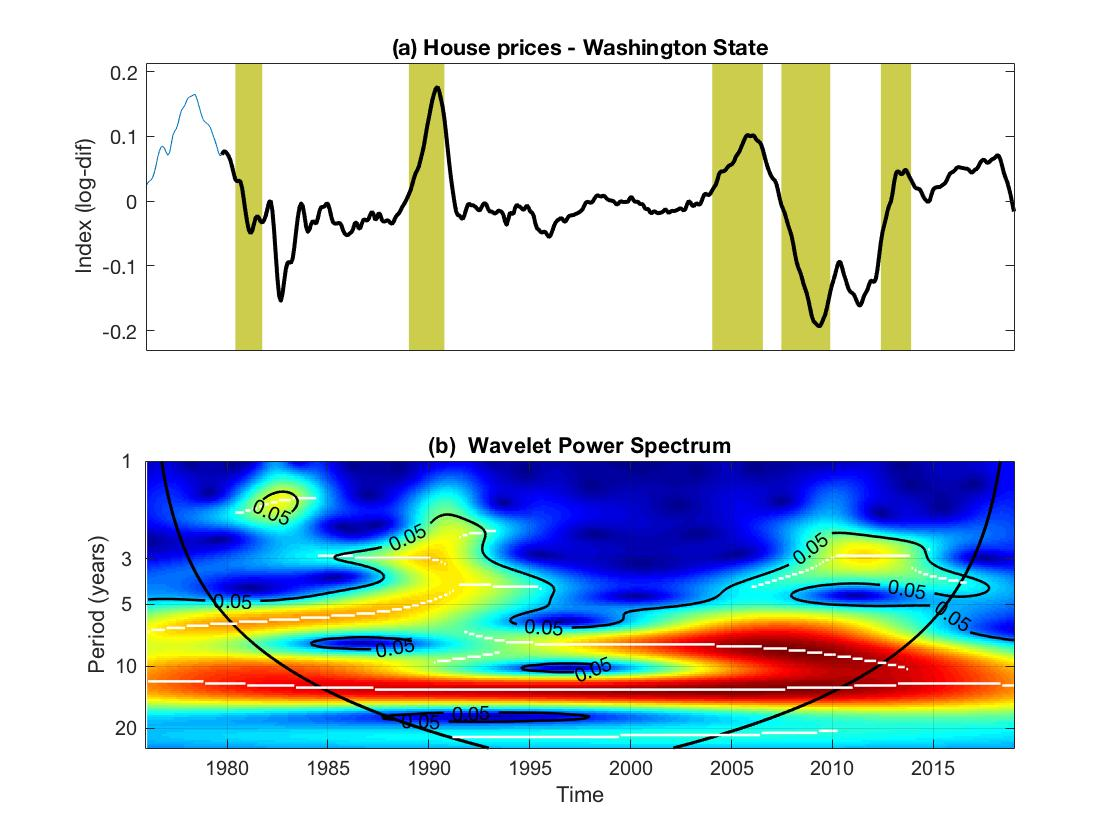
\includegraphics[width=1\linewidth]{figs/Fig_empiricalExample_washington.jpg}
\caption{This figure presents analysis of price data for Washington State as an example: (a) monthly price series where I have also shaded (green) 'bubble episodes' as identified by the PSY test \citep{Shi2016, Phillips2015} applied to these series; (b) the local wavelet power spectrum (Eq.\ref{eq:wps}) of this series (hot colours indicated regions of high power, cold colours areas of low power).}
\label{cycleExample1}
\end{figure}

\begin{figure}[tbh!]
\centering
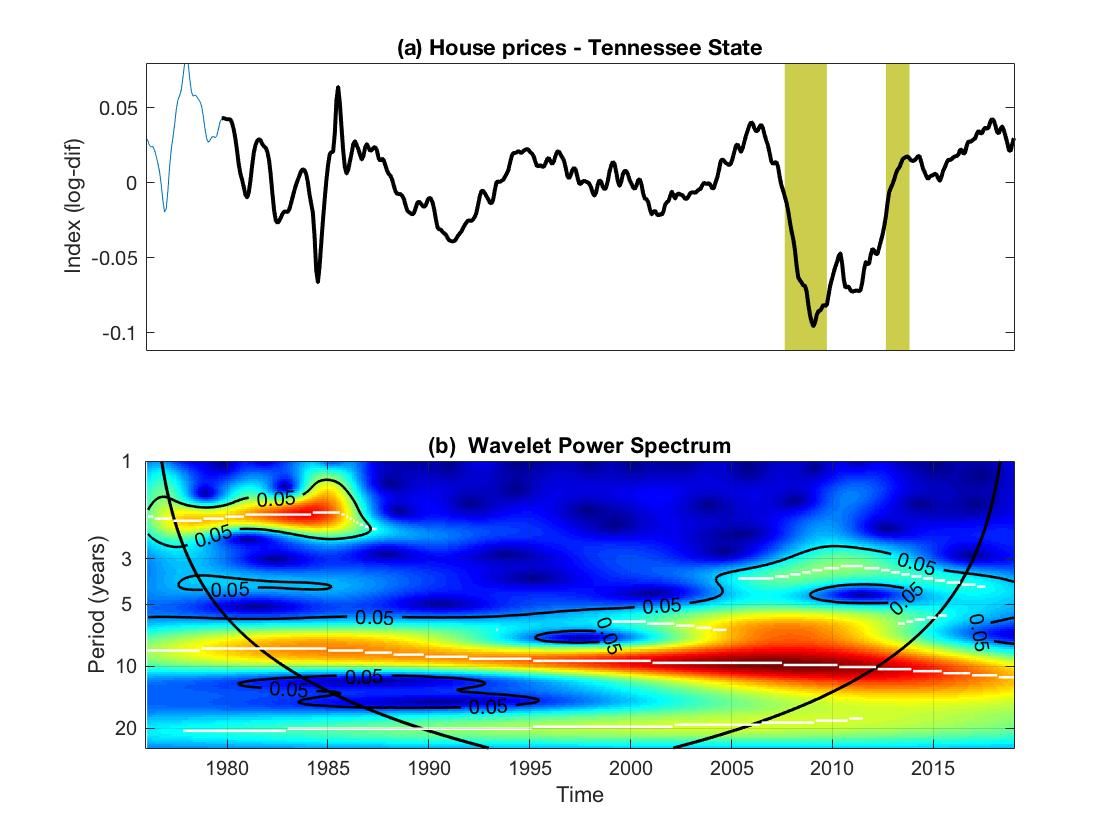
\includegraphics[width=1\linewidth]{figs/Fig_empiricalExample_tennessee.jpg}
\caption{This figure presents the same analysis as Fig.\ref{cycleExample1}, but taking  Tennessee as an example.}
\label{cycleExample2}
\end{figure}

These examples are by no means unusual. Strikingly, while a small minority of states show no significant evidence of a periodic component to house price fluctuations (Alaska, Mississippi, West Virginia); most exhibit clear evidence of well-defined permanent cycles. In many cases these periodic components are statistically significant (indicated by dark black contour lines in Fig.\ref{cycleExample1} and Fig.\ref{cycleExample2})\footnote{I test cycles in the wavelet spectrum against a null hypothesis that takes account of the highly auto-correlated character of house price series: statistical significance is assessed with Monte Carlo simulations - the distribution of the wavelet power spectrum under the null hypothesis is constructed based on the wavelet power spectrum of 1,000 surrogates, and the 95th percentile of this distribution extracted. Surrogates are obtained by fitting an ARMA(p,q) model to the series and constructing new samples by drawing errors from a Gaussian distribution.} %under the testing procedure [NOT EXPLAINED/INTRODUCED] employed 
(e.g. California, DC, Oregon, Washington), in others a spectral ridge, whilst not statistically significant under the testing procedure employed, is nevertheless a clearly visible feature of the power spectrum (e.g. Nebraska, Ohio, Texas).%\footnote{The interested reader is invited to inspect Appendix section \ref{} where (in the interests of space) the local power spectra for all $51$ series are exhaustively presented.}

%While not unusual for exhibiting non-zero frequency spectral ridges, these two examples do illustrate underlying  cycle dynamics that (i) are missed by tests for time-localised explosive behaviour and (ii) are also a feature of markers that do not exhibit `bubble episodes' at all.

All of these states appear to exhibit cycles of similar periodicity. This is clarified and summarized by Fig.\ref{periodicity} which presents the spectral ridges obtained for each state level price series (across all $51$ states) as (\textit{a}) a density plot in the time-frequency plane and also (\textit{b}) aggregated not only across states but also across time.

\begin{figure}[tbh!]
\centering
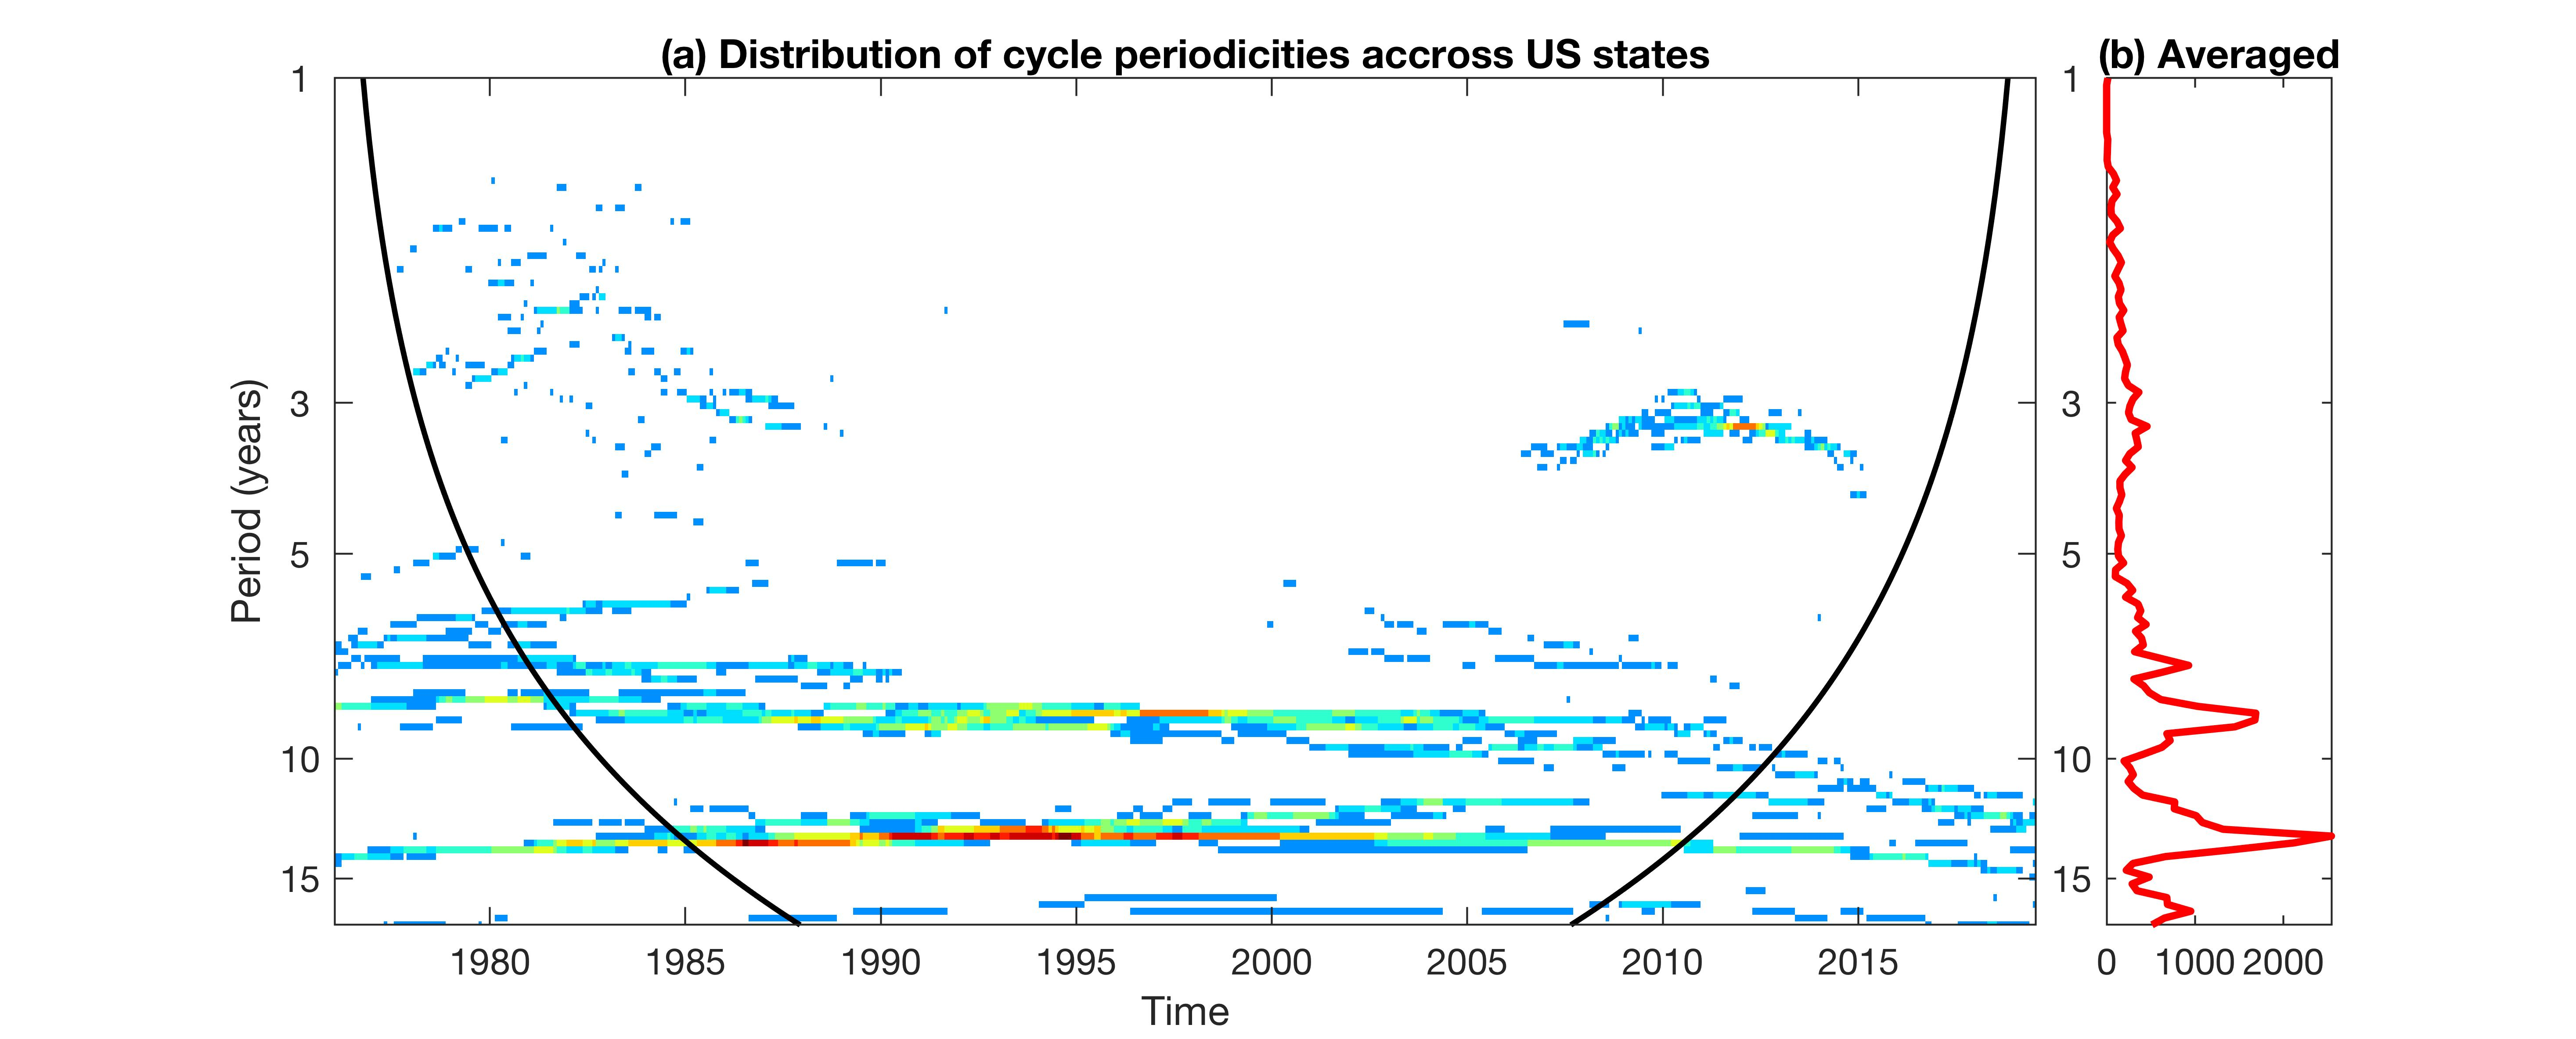
\includegraphics[width=1\linewidth]{figs/Fig_cycle_frequencies.jpg}
\caption{This figure presents the distribution of estimates of instantaneous cycle periodicity (given for individual states by the white lines in Fig.\ref{cycleExample1}-\ref{cycleExample2}), aggregated (\textit{a}) across all US states (colour represents the density, with hotter colours indicating higher density) and (\textit{b}) across both states and time, from 1975 to 2019.}
\label{periodicity}
\end{figure}

This analysis reveals that states across the U.S. share price cycles of remarkably similar periodicity - of %between 8 and 10 years (consistent with c.$5$ cycles over the nearly $50$ year sample period), 
about 9 years (consistent with c.$5$ cycles over the nearly $50$ year sample period) and of about 12 years (rather long relative to sample period c.$4$ cycles). This is clearly indicated by the two sharp peaks in the density in Fig.\ref{periodicity}:b and the time-frequency information provided by Fig.\ref{periodicity}:a (where the similarity of cycle frequencies shows up as two narrow and clearly separated bands).

We may also see evidence of the convergence of frequencies toward the lower frequency after 2006. Or it may be that the higher frequency cycle component dies out.\footnote{Caution is required over either interpretation given much of the relevant period is subject to edge effects.}

This result clearly indicates that these common cycles are not only a feature of the national bubble episode, but have existed across the entire sample period (where the crisis shows up is as a well defined local area of density around the 3 year periodicity band between 2006 and 2014 consistent with a time localised shock).

%%%%%%%%%%%%%%%%%%%%%%%%%%%%%%%%%%
\subsection{Phase coherence analysis reveals synchronisation of permanent state level cycles}

The presence of common cycles (in the sense of cycles with very similar periodicity) across most US states over the entire c.50 year sample period, seems to raise the question why this cycle was not more prominent in aggregate house price fluctuations before the 2000s. Implicitly we must assume these cycles cannot have been well synchronised (such that out of phase relationships moderated aggregate cyclicality).

%I use instantaneous phase series obtained as scale-band average from \ref{eq:phase} as a basis for dynamic measures of the  phase-synchronisation that could be used in order to study the time-evolution of synchronisation among common cycle components

The so called Kuramoto order parameter (Eq.\ref{eq:r}) provides a %simple and 
natural  and widely employed measure of phase synchronisation in a multivariate context.

\begin{equation}
 R(t)=r(t)e^{i\phi(t)}=\frac{1}{N}\sum_{j=1}^{N}e^{i\theta_{x_i}(t)}
 \label{eq:r}
\end{equation}

Here the statistics $r$ and $\phi$ provide a quantification of the collective dynamics and current state of the whole population, where the modulus $r=|R|$,  $0\leq{r}\leq{1}$ measures the phase coherence of the population (achieving its maximum $r=1$ when all phases are identical and its minimum $r=0$ when phases are balanced around the phase circle), thus provides a measure of the overall phase-synchrony in the system (without the need to define a reference cycle), and $\phi$ is the average phase (i.e. the vector R points in the average direction of all the $e^{i\theta_{x_i}}$ vectors). 

While this mean field order parameter (Eq.\ref{eq:r}) provides a measure of overall level of phase synchronisation across all markets relevant for the aggregate level, it does not provide local information. %It measures the average of the phase differences across all pairs of cycles.

Following \cite{Schroder2017} I define an alternative order parameter

\begin{equation}
 r_{uni}(t)=\frac{1}{\sum_{i=1}^{N}{k_i}}\sum_{i,j=1}^{N}A_{i,j}\mathfrak{R}\left(e^{i(\theta_{x_i}(t)-\theta_{x_j}(t))}\right)
 \label{eq:runi}
\end{equation}

By introducing a spatial adjacency matrix $A_{states}$ constructed based on the spatial contiguity of US states into Eq.\ref{eq:runi}, I am able to quantify phase-synchrony considering only the phase-differences between price cycles in neighbouring states. In order to assess \textit{local} synchronisation relative to the \textit{overall} level of synchronisation among markets, I obtain $r$ both for $A_{states}$ and based on the all-to-all network (equivalent to mean field analysis Eq.\ref{eq:r}).\footnote{I also use a random networks approach (randomly assigning links between states) to assess the question of how smooth change in phase-angles are over the spatial adjacency network compared to some random configuration of local links. This yields similar results.}

Since the instantaneous phase is obtained scale-by-scale, these statistics can be calculated for every scale at every time step, or by averaging over a specific scale band, it is possible to characterise overall phase relationships for differed frequency ranges and track the evolution of this over time.

Since the idea is to understand the time varying synchronisation among the common permanent cycle components identified in Fig.\ref{periodicity}, I obtain the phase series %as per Eq.\ref{eq:phase} 
averaged over the  8-12 year periodicity band identified as relevant by this analysis. \footnote{Phase-differences \(\theta_{x_{i_j}}=\theta{x_i}-\theta_{x_j}\) are obtained from \(\arctan{\left(\frac{\mathfrak{I}\{W_{x_{i_j};\psi} (a,\tau)\}}{\mathfrak{R}\{W_{x_{i_j};\psi} (a,\tau)\}}\right)}\) (where \(W_{x_{i_j};\psi}\) the wavelet cross-spectrum of two series) fully consistent with the individual phases (Eq.\ref{eq:phase}).}

Note this instantaneous phase based approach yields well time-resolved information in contrast with common approaches to phase and phase-synchronisation in the business cycle literature based on discrete points (turning points analysis) \citep{Harding2003,Harding2006,Harding2002}.

Fig.\ref{synch} presents the results of this analysis which provides clear evidence (i) that spatial adjacency matters for synchronisation (spatially adjacent markets have always been highly synchronous) and (ii) a dramatic increase in the global synchronisation of markets across the U.S. after 1995.

\begin{figure}[tbh!]
\centering
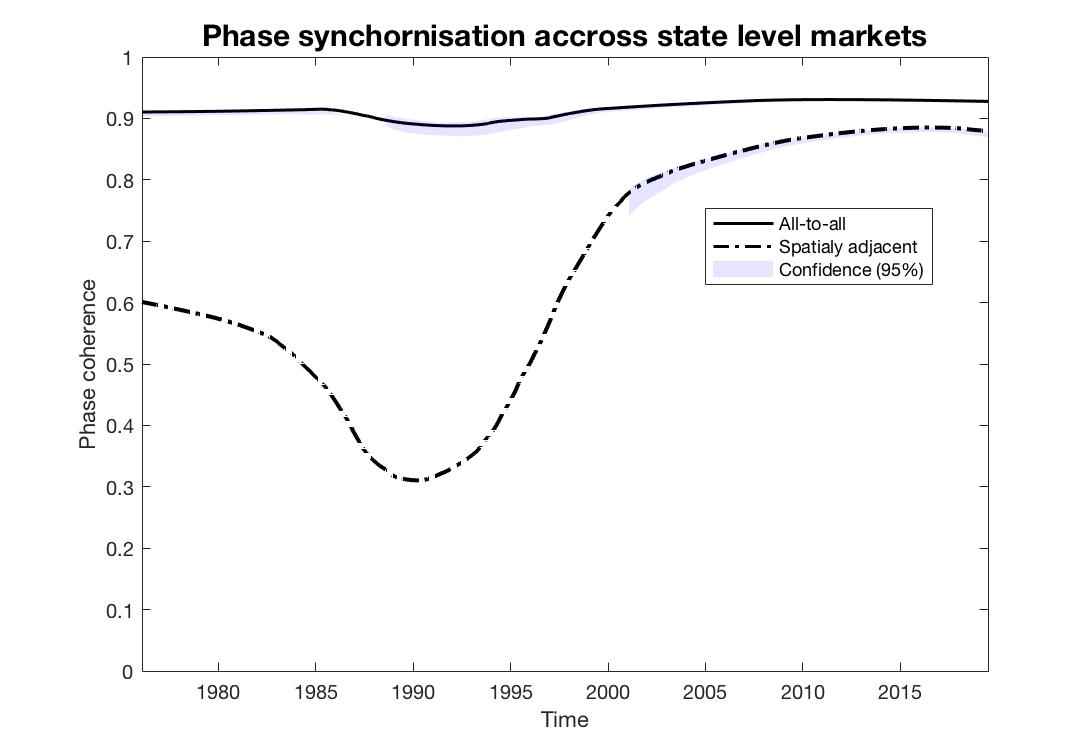
\includegraphics[width=1\linewidth]{figs/phase_coherence.jpg}
\caption{This figure presents the evolution over time of the local vs. global phase synchronisation of housing cycles across U.S. states (based on 8-12 year periodicity band of common cycle component) quantified as \ref{eq:runi} obtained, respectively, based on \textit{spatial adjacency} and \textit{all-to-all} networks.}
\label{synch}
\end{figure}

The implications for phase-synchronisation on aggregate cyclicality are illustrated by Fig.\ref{meanWPS} which compares the WPS (Eq.\ref{eq:wps}) of the mean price series; to the mean WPS of the 51 different price series (providing information on areas of common high power disregarding phase-shifts). This analysis clearly reveals common features of local house price series dynamics that are lost or obscured in the aggregated (average) time series. 

Of particular interest is the much more pronounced spectral ridge (cycle) that shows up in the mean spectrum Fig.\ref{meanWPS}:b and narrower band of high power even during the national boom-bust period. 

Another striking feature of the mean spectrum in Fig.\ref{meanWPS}:b is the very clear common shock showing up in the 2-4 year periodicity band during the early 1980s – something that entirely averages out according to the spectrum of mean house prices in Fig.\ref{meanWPS}:a.


\begin{figure}[tbh!]
\centering
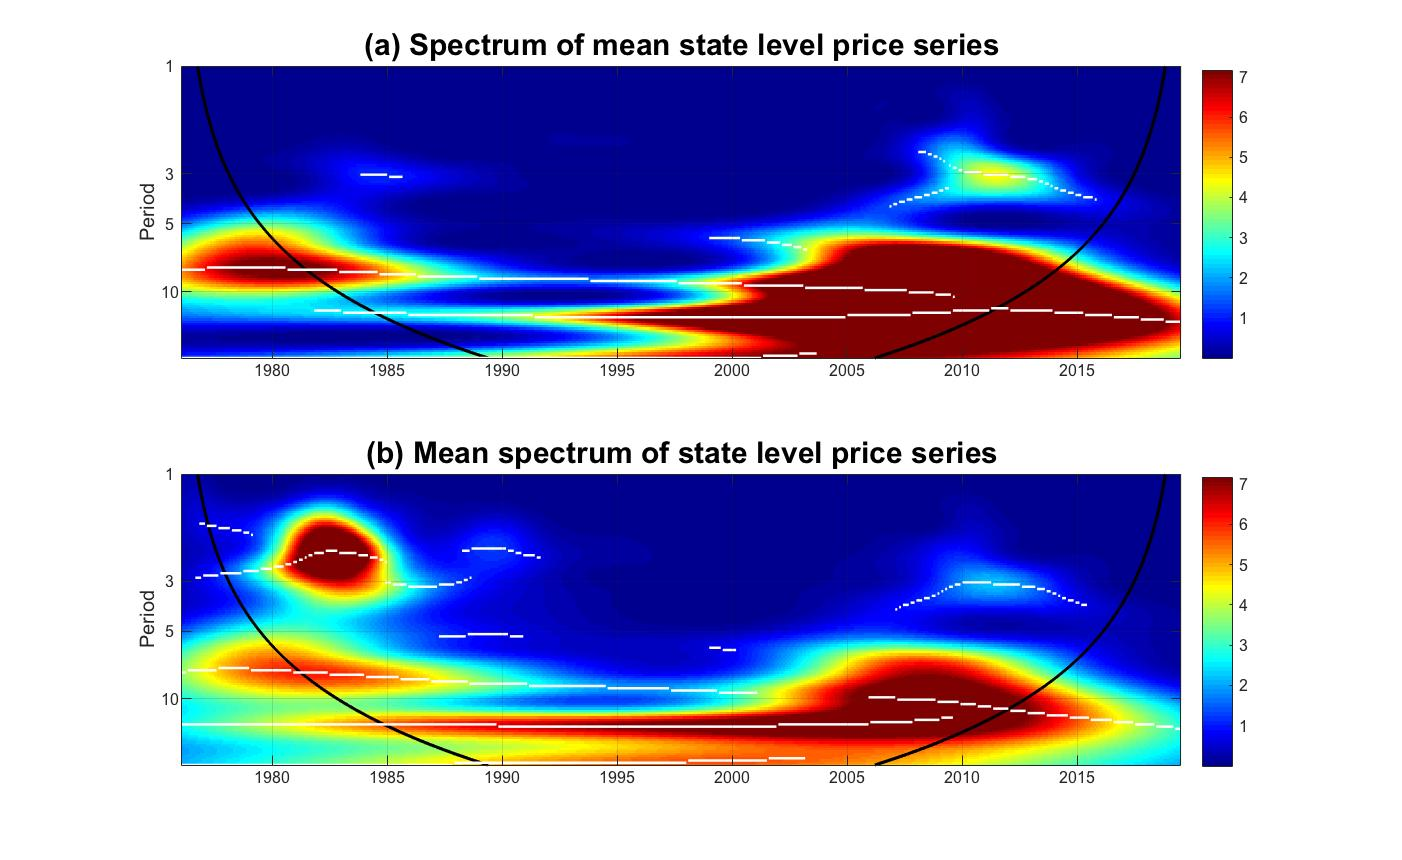
\includegraphics[width=1\linewidth]{figs/mean_wavelet_spectra.jpg}
\caption{This chart presents  (a) the wavelet spectrum of average house prices across all 51 states and DC; (b) the average power spectrum of all 51 states and DC (revealing areas of common high power disregarding phase-shifts).}
\label{meanWPS}
\end{figure}

These results clearly show the longstanding existence of a common cycle but that the contribution from this cycle to mean house price variation at the national
level was significantly moderated prior to the 2000s by the phase shifts between markets. However a dramatic increase in synchronisation after 1995 contributed to the subsequent national boom-bust.


\subsection{Spatial analysis reveals striking travelling-waves}

\begin{figure}[tbp!]
%\vspace{1.5cm}
\centering
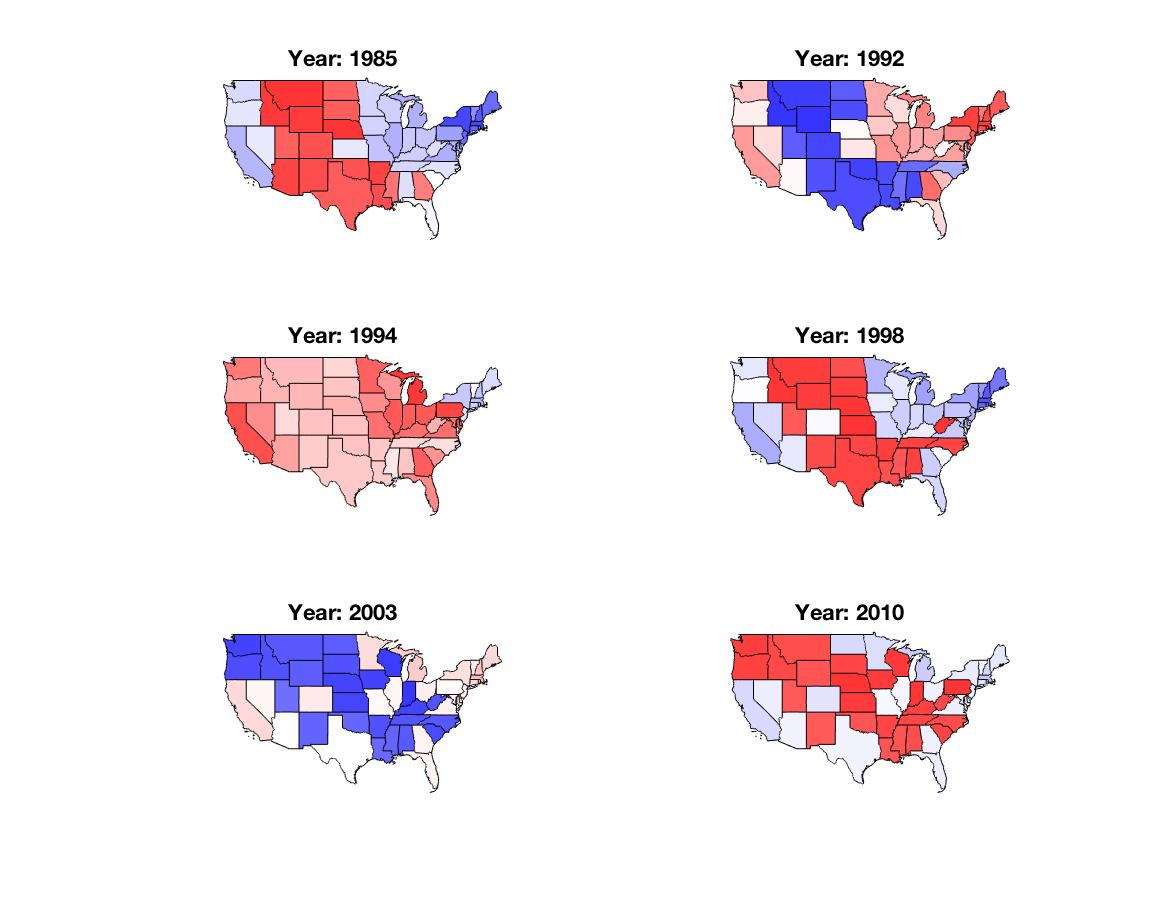
\includegraphics[width=0.97\textwidth]{figs/Fig_phase_heatmap_examples.jpg}
\caption{These heatmaps present the instantaneous phase of cycles in state level data across the US at six different points in time over the sample period. Here peak to trough is red increasing in intensity towards the trough, and trough to peak is blue, increasing in intensity towards the peak. This colour scheme makes a stark contrast between expansionary phase vs. contractionary phase cycles, but we also see e.g. in 1994 how the phase changes over space with coastal states close to troughing while central states are only just turning down. While these charts demonstrate the spatial patterns in relative phase, striking in the dynamic version, is how turning points ripple from adjacent state to adjacent state (e.g. another striking feature of the pre-2000s period in particular is the distinct segmentation of the northeast states).}
\label{ripple}
%\vspace{1.5cm}
%\vspace{1cm}
\end{figure}

An interesting and important question arises, whether low levels of overall synchronisation prior to 1995, may have concealed local synchronisation among markets (e.g. geographical clusters of synchronised markets), what is more whether the global synchronisation that occurred after 1995 was principally driven by common national factors, or whether local (in the sense of direct bilateral) links between individual markets could have played an important role. 

Moreover the strong evidence presented in Fig.\ref{synch} that spatial adjacency matters raises the question what sort of spatial patterns in the timing of state level housing cycles underpin this result? 

In order to understand the specific pattern of relationships between markets across the U.S. I make a spatial projection of the evolution of the instantaneous phase  series $\theta_{x_n}$ (Eq.\ref{eq:phase}) obtained for each of the 48 contiguous US states. This results in a dynamic heatmap. The idea is to explore whether there is any spatial pattern in the common cycle component identified in Fig.\ref{periodicity}. I thus look at scale averaged phase series for the 8-12 year periodicity band identified by this analysis.

The spatial projection of state level data allows me to assess not just whether neighbouring markets are more synchronous, but global patterns across markets, such as spatial segmentation (e.g. spatial clusters of synchronised markets or other spatial distribution of markets with similar phase); and the geographical distribution of leading and lagging markets and any propagation patterns of housing cycles across markets (such as ‘epicentre’ patterns reflecting the spatial diffusion of local shocks).

This dynamic heat-map clearly reveals a striking ‘travelling wave’ pattern: phase differences in price cycles in neighbouring states generate a periodic wave travelling across the US (analogous to a “Mexican wave”). Fig. \ref{ripple} illustrates the observed pattern using some point-in-time ‘snapshots’ from different dates over the sample period. Here I have used the intensity of blue (red) to express the deepening of expansionary (contractionary) phase of the cycle. The full dynamic heat-map visualisation (which is much more informative) is available \href{https://drive.google.com/open?id=1FMoofEgMtoN8mG1rMufnRmfiIVoV_c_d}{here}\footnote{Link to dynamic heatmap file: \url{https://drive.google.com/open?id=1FMoofEgMtoN8mG1rMufnRmfiIVoV_c_d}} and also provided in supplementary materials.
%\vspace{\extraspace}

In order to help assess the stability of/changes in this spatial pattern in the phase relationships between cycles, %I use a continuous measure quantifying the phase shift of each individual market with respect to the overall mean phase across all states at each time step:
I calculate the mean phase series $\phi$ across all markets from Eq.\ref{eq:r} then calculate the phase of each state relative to the mean phase across all sates (or relative phase angle (RPA)) as:

\begin{equation}
 \theta_{x_n,\phi}(t)=\theta_{x_n}(t)-\phi(t)
 \label{eq:rpa}
\end{equation}

This provides a continuous measure quantifying the phase shift of an individual market with respect to the overall collective development across states at each time-step.\footnote{Of course one problem with this approach is that the mean phase is not so meaningful when synchronisation is very low.} %This is defined for every state at every time step. 
Finally in order to provide a more succinct summary of the relationships identified for presentation here, I obtain the time averaged relative phase

\begin{equation}
 \bar{\theta}_{x_n,\phi}=\frac{1}{T}\sum_{t=1}^T{\theta_{x_n,\phi}(t)}
 \label{eq:mrpa}
\end{equation}

for all states for a series of  (non-overlapping) sub-periods (using a 10 year window). Fig. \ref{rpa} presents the results of this analysis.\footnote{Note that while as far as I am aware these sort of relative phase differences have not previously been employed in economics,  they have been used in a number of other applications \citep{Richardson2012,Lamb2014,Brouwer2013,Varlet2011}.}

%This analysis helps to show both the consistency in the spatial pattern of relative timings over time, as well as the national synchronisation accross markets: 

\begin{figure}[tbp!]
\vspace{1.5cm}
\centering
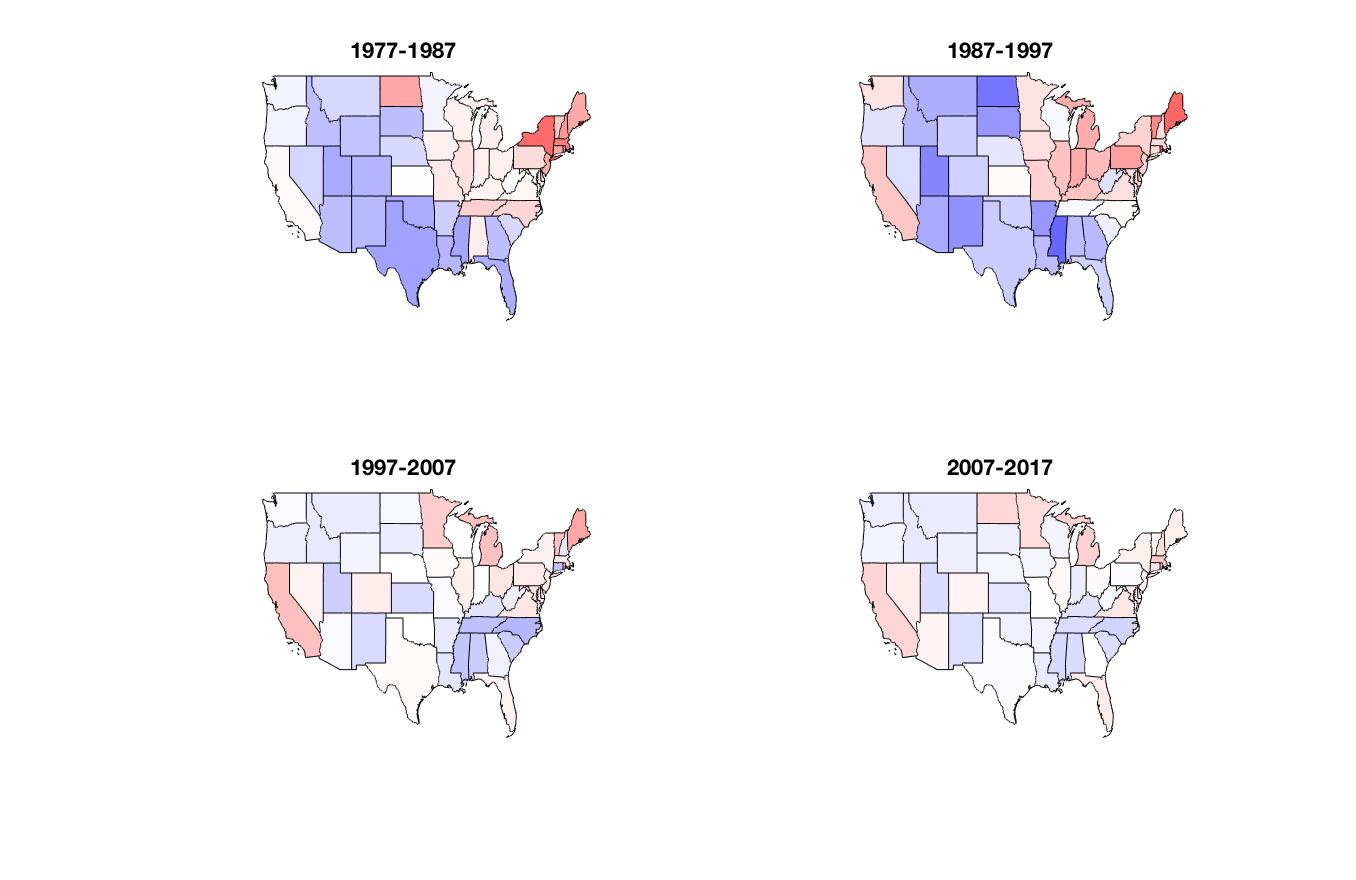
\includegraphics[width=0.97\textwidth]{figs/Fig_MRPA_subperiods.jpg}
\caption{These heat-maps plot the relative phases of each state averaged over four non-overlapping 10-year windows spanning most of the sample period. Here red means ahead of the mean phase and blue lagging the mean phase, meanwhile stronger colours indicate a larger lead or lag (colours are consistent between maps).}
\label{rpa}
\vspace{1.5cm}
\end{figure}

We see the general pattern of lead-lags is relatively stable over time with coastal states leading. However a number of changes are also apparent: (i) the distribution around the mean phase tightens in the second half of the sample (hence the lighter colours in 1997-2007 and 2007-21017 charts); (ii) the spatially segmented strongly leading cluster of states in the north east weakens in the second half of the sample period.


%%%%%%%%%%%%%%%%%%%%%%%%%%%%%%%%%%%%%%%%%%%%%%%%%%%%%%%%%%%%%%%%%%%%%%%%%%%%%%%%
\section{Interpretation and significance} \label{Discussion}

Many sub-national housing markets in the U.S. exhibit a long history of repeated boom-bust resembling an ongoing cycle. The dynamic character of these cycles represents an important question.

A series of random shocks could generate a ‘cycle’ in the sense of successive periods of expansion and contraction (closely analogous to modern business cycle theory) \citep{Bracke2013}; alternatively if markets are \say{bubbly} enough (i.e. if bubbles easily emerge but inevitably burst) this explosiveness could be the engine behind a cycle formed by a sequence of bursting bubbles \citep{Evans1991,Shi2007,Shi2017}.

The multiple bubbles hypothesis is empirically supported by evidence of temporarily explosive dynamics \citep{Shi2017,Hu2018,Greenaway-mcgrevy2015,Pavlidis2018} - the time series signature of an unstable bubble process (see \cite{Phillips2015} for an overview).

Whether cycles are being driven by successive shocks or bubbles, under this episodic view housing cycles might recur, but would be fundamentally \textit{irregular} and \textit{unpredictable}.  

On the contrary the stable spectral ridges exhibited by the majority of sub-national markets suggest that housing cycles - while they may exhibit \say{bubbly} behaviour - also have a cycle component with a preferred period.\footnote{This feature was missed by \cite{Flor2017} who only consider a shorter time series dimension and higher periodicity bands.}

The existence of a striking \textit{spatial-ripple} (not previously documented in the literature)\footnote{A considerable part of the \say{ripple} literature has relied on cointegration tests for convergence - studies for the U.S. report mixed but limited evidence of convergence for US markets and this has been argued to cast doubt on the existence of a \say{ripple effect} in the U.S. \citep{Clark2009,Gil-Alana2014,Barros2012,Gupta2012,Holly2010,Holmes2011,Pollakowski1997,Zohrabyan2008}.} in this common cycle component, provides strong evidence of some form of spatial dependence. However the \textit{stability} of this pattern over time seems furthermore, inconsistent with the sort of spatial diffusion of idiosyncratic shocks \citep{Barros2012, Holmes2011,Meen1996,Meen1999,Cook2003,Drake1995,Holly2010} or contagious bubbles \citep{Riddel2011,DeFusco2013,Nneji2015} commonly hypothesised in the real estate literature: random shocks to different markets at different times (or idiosyncratic random bubble episodes in different markets at different times), would tend to mean different states leading the national housing cycle at different times and changing lead-lag patterns across markets.

Perhaps if particular markets were key sources of shocks/bubbles, they might tend to dominate, generating a persistent pattern of lead-lags. Even so we might well expect both the spatial diffusion of random shocks or of contagious bubbles alike, to generate \textit{epicentre} diffusion patterns, and not the \textit{travelling-wave} pattern I documented in this analysis (Fig.\ref{ripple}-\ref{rpa}).

Indeed a subtle but possibly particularly revealing observation, is how the spatial pattern I document (see \ref{ripple} and \ref{rpa}) clearly shows cycle phase changing rather smoothly over space along one spatial projection (creating the \say{ripple effect}), and almost constant on the projection orthogonal to this - a pattern that characteristically arises in locally coupled cycle systems.

Taken together these results thus suggest an important role both for (i) local spatial coupling between markets and (ii) non-trivial intrinsic cycle dynamics, thus a possible dramatic re-interpretation of the character of U.S. housing market instability as the synchrony of a spatially coupled network of cycles.

In this setting, the possibility arises that the global synchronisation event could have been emergent (a widely observed phenomenon even for weakly coupled systems); alternatively it may have been triggered by the introduction of some new or stronger coupling between markets (resulting in a bifurcation). 

However, while the \textit{spatial-wave} provides clear evidence of spatial coupling, raising the possibility that the observed national synchronisation could have been an emergent outcome due to the local spatial interaction of cycles; it is equally plausible that the dramatic synchronisation event I document could have resulted from a significant common shock.

Indeed it is striking that the de-synchronisation period (1984-1995) coincides with the period of savings and loans company failures \citep{Green2005,Snowden1997} and follows some important common shock in the early 1980s revealed by the mean power spectrum (Fig.\ref{meanWPS}.b). What is more that the dramatic synchronisation after 1995 coincides with the deregulation of interstate banking (1995) and shift from local ‘balance sheet lending’ by depositories, to a national market based system of securitised mortgage finance \citep{Schnure2005}. 

These associations potentially suggest national financial factors - often cited as possible drivers by the national bubble hypothesis - may have played a significant role in the observed shifts in synchronicity (something likely to be of interest to an existing literature that has linked increased housing market correlation with financial integration in the U.S. \citep{Landier2017,Klyuev2008}). %However the shock driven synchronisation of permanent locally coupled cycles 

It is also interesting to note how the de-synchronisation period also coincides broadly with the ``Great Moderation" period.%, raising the question whether this de-synchronisation moderated spillovers or feedback between the housing cycle and the macroeconomy. % suggesting possibility that de-synchronisation moderated spillovers or feedback between housing cycle and the macroeconomy.


%%%%%%%%%%%%%%%%%%%%%%%%%%%%%%%%%%%%%%%%%%%%%%%%%%%%%%%%%%%%%%%%%%%%%%%%%%%%%%%%
\section{Conclusions} \label{conclusion}

In this paper I use time-frequency methods and the phase-amplitude decomposition facilitated by complex wavelet analysis, to study spatio-temporal patterns in U.S. housing market fluctuations. These methods allow me to study how the spectral structure of house price fluctuations and spatial patterns in the timing of cycles in different markets have evolved with time. 

The power and flexibility of these methods allows me to derive a series striking new results:

I document for the first time that house price fluctuations in markets all across the U.S. exhibit a clear spectral ridge (estimated as local maxima of wavelet power spectrum) consistent with a cyclical component with a preferred period. What is more cycles in different markets share a c.10 year periodicity. I show that historically phase-shifts between these cycles moderated aggregate house price cyclicality. However the global synchronisation of these existing cycles after 1995 contributed to the emergence of a national housing cycle.

Focusing on the scale band around the relatively well defined c.10 year cycle identified, I am able to generate a phase angle for each market at each (monthly) time step. With this phase information I am able to show that there exists a striking \textit{travelling-wave} pattern in the timing of U.S. housing market cycles (not previously documented). This pattern has been relatively stable over time and resembles patterns typically arising in networks of locally coupled cycles. Taken together these findings suggest an important role both for (i) local spatial coupling between markets and (ii) non-trivial intrinsic cycle dynamics leading to a possible re-interpretation of the character of U.S. housing market instability in terms of either emergent and/or common shock driven synchronisation of coupled cycles across a spatial network.

\section{Acknowledgments}
I gratefully acknowledge use of code from \href{https://sites.google.com/site/aguiarconraria/joanasoares-wavelets/the-astoolbox}{ASToolbox}\footnote{Available for download at: \url{https://sites.google.com/site/aguiarconraria/joanasoares-wavelets/the-astoolbox}} (See \cite{Aguiar-Conraria2014}) and code made available by Prof. Shuping Shi\footnote{Available for download at: \url{https://sites.google.com/site/shupingshi/home/codes}} in my analysis. While it is not possible to list everyone, I am also grateful to (among others) Dr. Robert Jump, Prof. Engelbert Stockhammer, Prof. Jagjit S. Chadha, Prof. Marcus Miller, Prof. Arnab Bhattacharjee, as well as participants in \textit{Bamberg Behavioural Economics Workshop}; \textit{NetSci Tokyo 2020} session on economic networks; and \textit{Bank of England} Macroeconomics Seminar for helpful comments and discussion. This work was funded by a Studentship from \textit{Kingston University London}.

%\section{Materials}

%Source code for CIFAR-10 supersampling experiments and a TensorFlow\cite{abadi2016tensorflow} implementation of ALRC is available at \url{\GitHubLoc}.

% ALRC increases the rate of convergence and decreases losses for otherwise unstable training by limiting loss spikes. If learning is already stable, it has little affect. Our algorithm is computationally inexpensive, robust to hyperparameter choices and can be applied to any loss function or batch size without affecting backpropagated gradient distributions. It follows that ALRC complements existing learning algorithms and can be applied to any artificial neural network trained with SGD.

%%%%%%%%%%%%%%%%%%%%%%%%%%%%%%%%%%%%%%%%%%%%%%%%%%%%%%%%%%%%%%%%%%%%%%%%%%%%%%%%

%\bibliographystyle{ieeetr}
%\bibliographystyle{dcu}
\bibliographystyle{plainnat}
%\bibliographystyle{not_plainnat}
%\bibliographystyle{humannat}
\bibliography{bibliography}


\clearpage

\end{document}
